% ---------------------------------------------------
% ----- Main document of the template
% ----- for Bachelor-, Master thesis and class papers
% ---------------------------------------------------
%  Created by C. Müller-Birn on 2012-08-17, CC-BY-SA 3.0.
%  Last upadte: C. Müller-Birn 2015-11-27
%  Freie Universität Berlin, Institute of Computer Science, Human Centered Computing.

\documentclass[pdftex,a4paper,12pt,DIV=calc,BCOR5mm,english,twoside,smallheadings,titlepage]{scrbook}
% ----- weitere Optionen
%draft,			% Entwurfsmodus zum Anzeigen zu leerer/voller Boxen
%DIV=calc
%DIV12,			% Seitengröße (siehe Koma Skript Dokumentation !)
%BCOR5mm,		% Zusätzlicher Rand auf der Innenseite
%twoside,		% Seitenränder werden an doppelseitig angepasst
%fleqn,			% Formeln werden linksbündig (und nicht zentriert) angezeigt
%titlepage,		% Titel wird in einer 'titlepage' Umgebung gesetzt
%bigheadings,	% Große Überschriften (normal, small-headings)
%halfparskip-	% Absatz wird nicht eingerückt, dafür aber um eine halbe Zeile nach unten gerückt
%
%---------------------------------------------------
%----- Packages
%---------------------------------------------------
%
\usepackage[T1]{fontenc}
\usepackage[utf8]{inputenc}
\usepackage[english]{babel}
\usepackage{ae}
\usepackage{bibgerm}

\usepackage{fancyhdr} % Define simple headings
\usepackage{xcolor}
\usepackage{url}
\usepackage{listings}
%\usepackage{vmargin} % Adjust margins in a simple way
%
\usepackage{amsmath}
%
\usepackage[pdftex]{graphicx}
\usepackage{hyperref} % turn all your internal references into hyperlinks
%\usepackage[pdfstartview=FitH,pdftitle={<<Titel der Arbeit>>}, pdfauthor={<<Autor>>}, pdfkeywords={<<Schlüsselwörter>>}, pdfsubject={<<Titel der Arbeit>>}, colorlinks=true, linkcolor=black, citecolor=black, urlcolor=black, hypertexnames=false, bookmarksnumbered=true, bookmarksopen=true, pdfborder = {0 0 0}]{hyperref}
%
% table settings
\usepackage{booktabs}
\usepackage{tabularx}
\usepackage{rotating}
\usepackage{longtable}
\usepackage{pdflscape}
\usepackage{multirow} %multi row
\usepackage{rotating} %for rotating table

\usepackage{verbatim}
\usepackage{longtable} % for multipage tables
\usepackage[stable]{footmisc} % for putting footnotes in section titles
%
%---------------------------------------------------
%----- PDF and document setup
%---------------------------------------------------
%
\hypersetup{
	pdftitle={You shall not publish: Edit filters on English Wikipedia},  % please, add the title of your thesis
    pdfauthor={<Author>},   % please, add your name
    pdfsubject={Master thesis, Institute of Computer Science, Freie Universität Berlin>}, % please, select the type of this document
    pdfstartview={FitH},    % fits the width of the page to the window
    pdfnewwindow=true, 		% links in new window
    colorlinks=false,  		% false: boxed links; true: colored links
    linkcolor=red,          % color of internal links
    citecolor=green,        % color of links to bibliography
    filecolor=magenta,      % color of file links
    urlcolor=cyan           % color of external links
}
%
%---------------------------------------------------
%----- Customize page size
%---------------------------------------------------
\usepackage[top=3cm,right=3cm,bottom=4cm,left=4cm]{geometry}
%
%---------------------------------------------------
%----- Customize header and footer\pagestyle{fancy}
%---------------------------------------------------
\pagestyle{fancy}

\fancyhf{}  % delete all existing header formating

\fancyhead[LE]{\leftmark}  % represent the current chapter heading in uppercase
\renewcommand{\chaptermark}[1]{ % adapt the shown chapter name: show it in lower case and with chapter number
\markboth{\thechapter.\ #1}{}}

\fancyhead[RO]{\rightmark}   % % represent the current section heading in uppercase
\renewcommand{\sectionmark}[1]{% adapt the shown section name: show it in lower case and with section number
\markboth{\thesection.\ #1}{}}

\renewcommand{\headrulewidth}{0pt} % remove lines from header
\renewcommand{\footrulewidth}{0pt} % remove lines from header

\fancyfoot{} % delete all existing footer formating
\fancyfoot[LE,RO]{\thepage} % put page number on the left on even page and right on odd page
%
%---------------------------------------------------
%----- Settings for word separation
%---------------------------------------------------
% Help for separation (from package babel, section 22)):
% In german package the following hints are additionally available:
% "- = an explicit hyphen sign, allowing hyphenation in the rest of the word
% "| = disable ligature at this position. (e.g., Schaf"|fell)
% "~ = for a compound word mark without a breakpoint (e.g., bergauf und "~ab)
% "= = for a compound word mark with a breakpoint, allowing hyphenation in the composing words
% "" = like "-, but producing no hyphen sign (e.g., und/""oder)
%
% Describe separation hints here:
\hyphenation{
% Pro-to-koll-in-stan-zen
% Ma-na-ge-ment  Netz-werk-ele-men-ten
% Netz-werk Netz-werk-re-ser-vie-rung
% Netz-werk-adap-ter Fein-ju-stier-ung
% Da-ten-strom-spe-zi-fi-ka-tion Pa-ket-rumpf
% Kon-troll-in-stanz
}
%
%---------------------------------------------------
%----- Restricting including files
%---------------------------------------------------
% Only files listed here will be included in the PDF document!
% In order to only partially translate the document, for example for bug-fixing,
% it might be useful to comment out some of the documents.
\includeonly{
title,
declaration,
abstract_en,
abstract_de,
preface,
introduction,
2-Background,
3-Methods,
4-Edit-Filters,
5-Overview-EN-Wiki,
6-Discussion,
conclusion,
%appendix
}

%%%%%%%%%%%%%%%%%%%%%%%%%%%%%%%%%%%%%%%%%%%%%%%%%%%%%%
% The content part of the documentent starts here! %%
%%%%%%%%%%%%%%%%%%%%%%%%%%%%%%%%%%%%%%%%%%%%%%%%%%%%%%

\begin{document}
%---------------------------------------------------
%----- Listing and color definition
%---------------------------------------------------
\definecolor{red}{rgb}{.8,.1,.2}
\definecolor{blue}{rgb}{.2,.3,.7}
\definecolor{lightyellow}{rgb}{1.,1.,.97}
\definecolor{gray}{rgb}{.7,.7,.7}
\definecolor{darkgreen}{rgb}{0,.5,.1}
\definecolor{darkyellow}{rgb}{1.,.7,.3}
\lstloadlanguages{C++,[Objective]C}
\lstset{
		escapeinside={§§}{§§},
        basicstyle=\ttfamily\footnotesize\mdseries,
        columns=fullflexible,% typewriter font look better with fullflex
        keywordstyle=\bfseries\color{blue},
%		identifierstyle=\bfseries,
        commentstyle=\color{darkgreen},
        stringstyle=\color{red},
        numbers=left,
        numberstyle=\ttfamily\scriptsize\color{gray},
%       stepnumber=5,
%       numberfirstline=true,
        breaklines=true,
%		prebreak=\\,
        showstringspaces=true,
        tabsize=4,
        captionpos=b,
%		framexrightmargin=-.2\textwidth,
        float=htb,
		frame=tb,
		frameshape={RYR}{n}{n}{RYR},
		rulecolor=\color{darkyellow},
        xleftmargin=15pt,
        xrightmargin=4pt,
        aboveskip=\bigskipamount,
        belowskip=\bigskipamount,
		backgroundcolor=\color{lightyellow},
		extendedchars=true,
       	belowcaptionskip=15pt
}

%---------------------------------------------------
%----- Title and declaration
%---------------------------------------------------
\pagenumbering{alph} % even though, these page numbers are not visible there are necessary to have unique page numbers
% ---------------------------------------------------
% ----- Title page of the template
% ----- for Bachelor-, Master thesis and class papers
% ---------------------------------------------------
%  Created by C. Müller-Birn on 2012-08-17, CC-BY-SA 3.0.
%  Freie Universität Berlin, Institute of Computer Science, Human Centered Computing.
%
\begin{titlepage}

\title{\includegraphics[width=0.6\textwidth]{pics/FU_logo.pdf}\\
{\small Master Thesis at the Computer Science Department of the Freie Universität Berlin}\\
{\small Human-Centered Computing (HCC)}\\
[6ex]
{\LARGE You shall not publish: Edit filters on English Wikipedia}}

\author{
{\emph{\normalsize<Ihr Vor- und Nachname>}}\\
{\normalsize Matrikelnummer: <IhreMatrikelnummer>}\\
{\normalsize <ihreemail@adresse.de>}\\
[18ex]
{\normalsize Supervisor and first examiner: Prof. Dr. Claudia Müller-Birn} \\
{\normalsize Second Examiner: Prof. Dr. Lutz Prechelt}}
\vspace{6ex}
\date{\normalsize Berlin, 25.07.2019}

\maketitle

\end{titlepage}

% ---------------------------------------------------
% ----- Declaration of the template
% ----- for Bachelor-, Master thesis and class papers
% ---------------------------------------------------
%  Created by C. Müller-Birn on 2012-08-17, CC-BY-SA 3.0.
%  Freie Universität Berlin, Institute of Computer Science, Human Centered Computing. 
%
\pagestyle{empty}

\subsection*{Eidesstattliche Erklärung}

Ich versichere hiermit an Eides Statt, dass diese Arbeit von niemand anderem als meiner Person verfasst worden ist. Alle verwendeten Hilfsmittel wie Berichte, Bücher, Internetseiten oder ähnliches sind im Literaturverzeichnis angegeben, Zitate aus fremden Arbeiten sind als solche kenntlich gemacht. Die Arbeit wurde bisher in gleicher oder ähnlicher Form keiner anderen Prüfungskommission vorgelegt und auch nicht veröffentlicht.
\par\bigskip  
\noindent Berlin, den \today

\vspace{1.2cm}

\noindent <Name>  

\cleardoublepage

%---------------------------------------------------
%----- Abstracts in English and German
%---------------------------------------------------

% ---------------------------------------------------
% ----- Abstract (English) of the template
% ----- for Bachelor-, Master thesis and class papers
% ---------------------------------------------------
%  Created by C. Müller-Birn on 2012-08-17, CC-BY-SA 3.0.
%  Freie Universität Berlin, Institute of Computer Science, Human Centered Computing.
%
\pagestyle{empty}

\subsection*{Abstract}

The present thesis offers a first investigation of one of Wikipedia's quality control mechanisms–edit filters.
It is analysed how edit filters fit in the quality control system of English Wikipedia, why they were introduced and what tasks they take over.
Moverover, it is discussed why rule based systems seem to be still popular today, when more advanced machine learning methods are available.
It was found that edit filters seem to be responsible for obvious but persistent types of vandalism, gladly disallowing these from the start so that (human) resources can be used more efficiently elsewhere (i.e. for judging less obvious cases).
In addition to disallowing this vandalism, edit filters appear to be applied in ambiguous situations where an edit is disruptive but motivation of the editor is not clear.
In such cases, the filters take an ``assume good faith'' approach and seek via warning messages to guide the disrupting editor towards transforming their contribution to a constructive one.
There are also a smaller number of filters taking care of haphazard maintenance tasks–above all tracking a certain bug or other behaviour for further investigation.
Finally, a comprehensive list of open questions for future research is compiled.

\begin{comment}
Include
- the topic of this thesis,
- important contents,
- results of your research
- and an evaluation of your results.
\end{comment}

\cleardoublepage

% ---------------------------------------------------
% ----- Abstract (German) of the template
% ----- for Bachelor-, Master thesis and class papers
% ---------------------------------------------------
%  Created by C. Müller-Birn on 2012-08-17, CC-BY-SA 3.0.
%  Freie Universität Berlin, Institute of Computer Science, Human Centered Computing. 
%
\pagestyle{empty}

\subsection*{Zusammenfassung}

<Hier sollten Sie eine kurze, aussagekräftige Zusammenfassung (ca. eine Seite) Ihrer Arbeit geben, welche das Thema der Arbeit, die wichtigsten Inhalte, die Arbeitsergebnisse und die Bewertung der Ergebnisse umfasst.> 

\cleardoublepage

%---------------------------------------------------
%----- Directories
%---------------------------------------------------

\frontmatter
\pagenumbering{roman}

\tableofcontents
\setcounter{tocdepth}{3}   % reduce the included sections in the table of content

\listoffigures
\listoftables

%---------------------------------------------------
%----- Main part
%---------------------------------------------------
\mainmatter
\pagenumbering{arabic}
\pagestyle{fancy}

% ---------------------------------------------------
% ----- Preface of the template
% ----- for Bachelor-, Master thesis and class papers
% ---------------------------------------------------
%  Created by C. Müller-Birn on 2012-08-17, CC-BY-SA 3.0.
%  Freie Universität Berlin, Institute of Computer Science, Human Centered Computing.
%
\chapter*{Vorwort}
\label{chap:preface}

\section*{Allgemeine Hinweise zur Erstellung einer Abschlussarbeit}

\begin{itemize}
	\item Beachten Sie, dass diese Vorlage für einen zweiseitigen Ausdruck angelegt wurde.
	\item Über die Papierqualität können Sie entscheiden, aber wir empfehlen aber Seiten mit wichtigen, farbigen Grafiken auch in Farbe auszudrucken und dabei ein höherwertiges Papier zu verwenden.
	\item Bitte stimmen Sie mit dem Betreuer Ihrer Arbeit auch den Zweitgutachter ab. Die Anfrage des Zweitgutachters erfolgt von Ihnen. Es ist an dieser Stelle sinnvoll, die Anfrage mit einer kurzen Zusammenfassung der Arbeit zu stellen.
	\item Bitte beachten Sie, dass Sie Ihre Abschlussarbeit mit einer Klebebindung versehen, eine Ringbindung ist nicht erwünscht.
\end{itemize}


% ---------------------------------------------------
% ----- Introduction of the template
% ----- for Bachelor-, Master thesis and class papers
% ---------------------------------------------------
%  Created by C. Müller-Birn on 2012-08-17, CC-BY-SA 3.0.
%  Last upadte: C. Müller-Birn 2015-11-27
%  Freie Universität Berlin, Institute of Computer Science, Human Centered Computing.
%
\chapter{Introduction}
\label{chap:introduction}

``Code 2.0 TO WIKIPEDIA, THE ONE SURPRISE THAT TEACHES MORE THAN EVERYTHING HERE.'' reads one of the inscriptions of Lawrence Lessig's ``Code Version 2.0'' (p.v)~\cite{Lessig2006}.
And although I'm not quite sure what exactly Lessig meant by this regarding the update of his famous book, I readily agree that Wikipedia is important because it teaches us stuff.
Not only in the literal sense, because it is, well, an encyclopedia.
Being an open encyclopedia, which has grown to be one of the biggest open collaborative projects in the world, studying its complex governance, community building and algorithmic systems can teach us a lot about other, less open systems.

%TODO verify all these claims and numbers
Since its conception in 2001, when nobody believed it was ever going to be a serious encyclopedia, the project has grown steadily.
At the latest, with the exponential surge in the numbers of users and edits around 2006, the community began realising that they needed a more automated quality control process.
The same year, the first anti vandal bots were introduced, followed by semi-automated tools such as Twinkle (in 2007) and Huggle (in the beginnings of 2008).
In 2009, yet another mechanism was introduced(syn)/announced/implemented.
Its core developer, Andrew Garrett, known on Wikipedia as User:Werdna, has called it ``abuse filter'', and according to EN Wikipedia's newspaper, The Signpost, its purpose was to ``allow[] all edits to be checked against automatic filters and heuristics, which can be set up to look for patterns of vandalism including page move vandalism and juvenile-type vandalism, as well as common newbie mistakes''.
%TODO decide whether to cite the Signpost here already, since it appears again in chapter4

\begin{comment}
Don't make it a separate subsection, but use it to introduce the topic with a story, the way Geiger does.
If the genesis doesn't make sense here, move it to Edit filters
\end{comment}

%************************************************************************
\section{Subject and Context}
%TODO should this be its own section? Or rather a part of next one?
\begin{itemize}
	\item Wo setze ich an? (Problemstellung / Ausgangslage)
	\item Identifikation der signifikanten Problemen im betrachteten Forschungsbereich
	\item Ein kurzer Überblick über den aktuellen Forschungsstand in dem Bereich inklusive vorhandener Lösungen (ausführlicher dann in den Folgeabschnitten)
\end{itemize}
%************************************************************************

The aim of the present work is to provide a comprehensive overview of Wikipedia's abuse filter extension, which was later renamed so that its end user facing part is nowadays known as Edit Filter.


This inquiry can be embedded in the context of (algorithmic) quality-control mechanisms on Wikipedia.
There is a whole ecosystem (syn?) of actors struggling to maintain the anyone-can-edit encyclopedia as good^^ and free of malicious, spam and ?(hoax?) content as possible.
We want to be able to better understand the role of edit filters in the vandal fighting network of humans, bots, semi-automated tools, and the machine learning framework ORES.
%After all, edit filters were introduced to Wikipedia at a time when bots and semi-automated tools already existed and were involved in quality control: in 2009 (compare timeline, Twinkle's page is from Jan 2007, Huggle's from beginning of 2008; bot's have been around longer, but first records, at least by me so far, of vandal fighting bots come from 2006 ). %TODO: when was the other stuff introduced
Why were filters introduced, when other mechanisms existed already?

Moreover, there seems to be a gap in the scientific literature on the subject.

\section{Aims of this work}
%alt title: \section{Intended Contributions}
%Epistemological interest

The aim of this work is to find out why edit filters were introduced on Wikipedia and how these fit in Wikipedia's quality control ecosystem.
More precisely, we want to unearth the tasks taken over by filters in contrast to other quality control meachanisms
and understand how different users of Wikipedia (admins/sysops, regular editors, readers) interact with these and what repercussions the filters have on them.
To this end, we study the academic contributions on Wikipedia's quality control mechanisms and give a descriptive overview of the adoption process as well as the current state of edit filters on EN Wikipedia.


\begin{comment}
Questions from Confluence
  Q1 We wanted to improve our understanding of the role of filters in existing algorithmic quality-control mechanisms (bots, ORES, humans).
  Q2 Which type of tasks do these filters take over in comparison to the other mechanisms? How these tasks evolve over time (are they changes in the type, number, etc.)?
  Q3 Since filters are classical rule-based systems, what are suitable areas of application for such rule-based system in contrast to the other ML-based approaches.

Note:
* to answer the question about evolution over time, I really do need the abuse_filter_history table
* modify 3rd question to: why are regexes still there when we have ML; answering it most probably involves talking to people
* check what questions the first bot papers asked, may serve as inspiration

\begin{itemize}
	\item Was sind die mit dieser Arbeit verfolgten Ziele? Welches Problem soll gelöst werden?
	\item Eine Beschreibung der ersten Ideen, der vorgeschlagene Ansatz und die aktuell erreichten Resultate
	\item Eine Beschreibung, welchen Beitrag die Arbeit leistet, um das vorgestellte Problem zu lösen
	\item Eine Diskussion, wie die vorgeschlagene Lösung sich von bestehenden unterscheidet, was ist neu oder besser?
\end{itemize}

* Think about: what's the computer science take on the field? How can we design a "better"/more efficient/more user friendly system? A system that reflects particular values (vgl Code 2.0, Chapter 3, p.34)?
  * GT is good for tackling controversial questions: e.g. are filters with disallow action a too severe interference with the editing process that has way too much negative consequences? (e.g. driving away new comers?)
\end{comment}

%TODO die wichtigsten erkenntnisse mehrmals erwähnen: intro, schluss, tralala; nicht dass sie unter gehen weil ich von lautern Bäumen den Wald nicht mehr sehe

* where is the thesis going?
  * should there be some recommended guidelines based on the insights?
  * or some design recommendations?
  * or maybe just a framework for future research: what are questions we just opened?; we still don't know the answer to and should be addressed by future research?

%************************************************************

\section{Methods}
\begin{itemize}
	\item Wie will ich meine Ziele erreichen? (Methodische Überlegungen)
	\item Darstellung zum Forschungsdesign.
	\item Insbesondere bei Master: Wie kann die Zielerreichung ``gemessen'' werden?
\end{itemize}

* methodology: what are the sources of knowledge
  * literature: what insights have we won from it?
  * documentation (Wikipedia, MediaWiki pages): what have we learnt here
  * data (filters stats, REGEX patterns): what do the filters actually do?

\section{Structure}

The remaining part of this thesis is organised in the following manner:
Chapter~\ref{chap:background} situates the topic in the academic discourse and examines some key notions relevant for the subsequent analysis.
In chapter~\ref{chap:methods}, I discuss scientific methods that helped me to accomplish the analysis (syn!).
Next, I describe the edit filter mechanism in general: how and why it was conceived, how it works and how it can be embedded in Wikipedia's quality control frame.
A detailed analysis (syn!) of the current state of all implemented edit filters on English Wikipedia is presented in chapter~\ref{chap:overview-en-wiki}.
We discuss the findings and the limitations of the inquiry in chapter~\ref{chap:discussion}.
Finally, the analysis (syn!) is wrapped up in the conclusion where also directions for possible future investigations are given.


\chapter{Background}
\label{chap:background}

\section{Vandalism on Wikipedia}

According to Wikipedia's newspaper, the Signpost, edit filters were initially introduced as a vandalism prevention mechanism (one of several)~\cite{Signpost2009}.
The aim of this section is to provide a better understanding of vandalism on Wikipedia. (What is vandalism, and what not; who engages in vandalism; who is striving to prevent it and with what means)

%What is vandalism

According to EN Wikipedia's policy~\cite{Wikipedia:Vandalism}, vandalism means ``intentionally making abusive edits to Wikipedia'' or, more specifically ``editing (or other behavior) deliberately intended to obstruct or defeat the project's purpose, which is to create a free encyclopedia''.
Vandalism includes ``malicious removal of encyclopedic content, or the changing of such content beyond all recognition, without any regard to our core content policies of neutral point of view (which does not mean no point of view), verifiability and no original research''
as well as ``adding irrelevant obscenities or crude humor to a page, illegitimately blanking pages, and inserting obvious nonsense into a page''
and ``[a]busive creation or usage of user accounts and IP addresses''.

Wikipedians have elaborated a whole vandalism typology(?).

%What is not vandalism

Disruptive editing

%Who engages in vandalism (and why?)

%Who is striving to prevent vandalism? How do they go about it?

Since Wikipedia is a ``do-it-yourself'' project, every editor who notices vandalism is called upon to help fixing it.
There is a formal process for reporting users who engage in vandalism %TODO look up Administrator intervention against vandalism
and requesting page protection for frequently vandalised pages. %TODO quote
And there are also users who specifically dedicate substantial amount of their Wikipedia contributions to fighting vandalism.

These dedicated vandal fighters mostly do so with the aid of some (semi or fully) automated tools which significally speeds up the process (see below).

\url{https://en.wikipedia.org/wiki/Wikipedia:Vandalism}

Consequences of vandalism, vandalism management
"Vandalism is prohibited. While editors are encouraged to warn and educate vandals, warnings are by no means a prerequisite for blocking a vandal (although administrators usually only block when multiple warnings have been issued). "

"Even if misguided, willfully against consensus, or disruptive, any good-faith effort to improve the encyclopedia is not vandalism."
"For example, edit warring over how exactly to present encyclopedic content is not vandalism." !!!
"Careful consideration may be required to differentiate between edits that are beneficial, edits that are detrimental but well-intentioned, and edits that are vandalism."
"If it is clear that the editor in question is intending to improve Wikipedia, those edits are not vandalism, even if they violate some other core policy of Wikipedia."
"When editors are editing in good faith, mislabeling their edits as vandalism makes them less likely to respond to corrective advice or to engage collaboratively during a disagreement,"

Handling
"Upon discovering vandalism, revert such edits, using the undo function or an anti-vandalism tool. Once the vandalism is undone, warn the vandalizing editor. Notify administrators at the vandalism noticeboard of editors who continue to vandalize after multiple warnings, and administrators should intervene to preserve content and prevent further disruption by blocking such editors. Users whose main or sole purpose is clearly vandalism may be blocked indefinitely without warning."

"examples of suspicious edits are those performed by IP addresses, red linked, or obviously improvised usernames"

One of the strategies to spot vandalism is "Watching for edits tagged by the abuse filter. However, many tagged edits are legitimate, so they should not be blindly reverted. That is, do not revert without at least reading the edit."

"Warn the vandal. Access the vandal's talk page and warn them. A simple note explaining the problem with their editing is sufficient. If desired, a series of warning templates exist to simplify the process of warning users, but these templates are not required."

Types of vandalism \url{https://en.wikipedia.org/wiki/Wikipedia:Vandalism#Types_of_vandalism}:
  (Abuse of tags; Account creation, malicious; Avoidant vandalism; Blanking, illegitimate; Copyrighted material, repeated uploading of; Edit summary vandalism; Format vandalism; Gaming the system; Hidden vandalism; Hoaxing vandalism; Image vandalism; Link vandalism; Page creation, illegitimate; Page lengthening; Page-move vandalism; Silly vandalism; Sneaky vandalism; Spam external linking; Stockbroking vandalism; talk page vandalism; Template vandalism; User and user talk page vandalism; Vandalbots;)

\url{https://en.wikipedia.org/wiki/Wikipedia:Disruptive_editing}

"Disruptive editing is not vandalism, though vandalism is disruptive."
"Disruptive editing is not always intentional. Editors may be accidentally disruptive because they don't understand how to correctly edit, or because they lack the social skills or competence necessary to work collaboratively "
Okay what are disruptive edits that are not vandalism? (apart from edit wars)

"sometimes attracts people who seek to exploit the site as a platform for pushing a single point of view, original research, advocacy, or self-promotion."
"not verifiable through reliable sources or insisting on giving undue weight to a minority view."

"Collectively, disruptive editors harm Wikipedia by degrading its reliability as a reference source and by exhausting the patience of productive editors who may quit the project in frustration when a disruptive editor continues with impunity."

examples of disruptive editing:
"Engages in "disruptive cite-tagging"; adds unjustified {{citation needed}} tags to an article when the content tagged is already sourced, uses such tags to suggest that properly sourced article content is questionable."
"Rejects or ignores community input: resists moderation and/or requests for comment, continuing to edit in pursuit of a certain point despite an opposing consensus from impartial editors."


\section{Quality-control mechanisms on Wikipedia}
%Context
Context of work: algorithmic quality-control mechanisms (bots, ORES, humans) -> filter?

%TODO Literature review!
Distinction filters/Bots: what tasks are handled by bots and what by filters (and why)? What difference does it make for admins? For users whose edits are being targeted?

socio-technical assemblages (see Geiger)

* Huggle, Twinkle, AWB, Bots exist nearly since the very beginning (2002?), why did the community introduce filters in 2009?

\subsection{Humans}

Some of the quality control work is done ``manually'' by humand editors.
That means, they engage in the standard encyclopedia editing mechanism (click the ``edit'' button on an article, enter changes in the editor which opens, write an edit summary for the edit, click ``save'') rather than using further automated tools to aid them.
According to research focusing on vandalism fighting, the amount/share/proportion of editors who engage in counter-vandalism measures that way shrinks in favour of semi or fully automated tools. %TODO quotes!
* what part of the quality control work do humans take over? (in contrast to the algorithmic mechanisms)

\url{https://en.wikipedia.org/wiki/Wikipedia:Recent_changes_patrol}

\subsection{Semi-automated tools}

Huggle, Twinkle, STiki~\cite{WestKanLee2010}
\url{http://en.wikipedia.org/wiki/Wikipedia:STiki}

\url{https://en.wikipedia.org/wiki/Wikipedia:AutoWikiBrowser}

\url{https://en.wikipedia.org/wiki/User:Lupin/Anti-vandal_tool}
"Please be aware that the original author of AVT (Lupin) is no longer active on Wikipedia. The script is very old and might stop working at any time."
"By using the RC feed to check a wiki-page's differences against a list of common vandal terms, this tool will detect many of the commonly known acts of online vandalism. "

\cite{GeiHal2013}
"Huggle, the most widely-used, fully assisted, counter-
vandalism tool, were made within 1 minute of the
offending edit. It is interesting that reverts with STiki, a
newer and more sophisticated queue-based vandal fighting
tool, are more often made to somewhat older edits, with a
time-to-revert distribution that is closer to unassisted edits.
This suggests that Huggle and STiki are targeting different
kinds of edits"

They also suggest that Twinkle (on one side) and Huggle and STiki are not in the same class of semi-automated vandal fighting tools, with Twinkle beeing more "manual" than the other 2.

VandalProof~\cite{HalRied2012}

"Huggle, one of the most popular
antivanda lism editing tools on
Wikipedia, is written in C#.NET
and any user can download and
install it. Huggle lets editors roll back
changes with a single mouse click,
but because the tool is so powerful,
rollback permission is restricted to
administrators and a few thousand
other Wikipedia users."
"Huggle makes it easy to review
a series of recent revisions by
filtering them according to the
user’s preferences."~\cite{HalRied2012}

huggle also sends out warnings to the offending editor on revert~\cite{HalRied2012}

\subsection{Bots}

ClueBot NG
"ClueBot_NG uses state-of-the-art machine learning techniques to review all contributions to
articles and to revert vandalism,"~\cite{HalRied2012}
XLinkBot
"XLinkBot reverts contributions that create links to
blacklisted domains as a way of quickly and permanently dealing with spammers."~\cite{HalRied2012}
HBC AIV Helperbots and MartinBot
"AIV Helperbot turns a simple page into a dynamic
priority-based discussion queue to support administrators in their work of identifying and
blocking vandals"~\cite{HalRied2012}

AntiVandalBot~\cite{HalRied2012}

Bots not patrolling constantly but instead doing batch cleanup works~\cite{GeiHal2013}:
AWB, DumbBOT, EmausBot
(also from figures: VolkovBot, WikitanvirBot, Xqbot)

\subsection{ORES}

%\section{Harassment and bullying}

\section{Algorithmic Governance}

maybe move it to edit filters chapter

\begin{itemize}
    \item Hier sollte enthalten sein, welche Anwendungen in diesem Bereich bereits existieren und warum bei diesen ein Defizit besteht.
    \item Falls genutzt, sollten hier die entsprechenden Algorithmen erläutert werden.
    \item Es sollten die Ziele der Anwendungsentwicklung, d.h. die Anforderungen herausgearbeitet werden. Dabei sollte die bestehende Literatur geeignet integriert werden.
\end{itemize}
 %Vandalism, Alg. quality control mechanisms, what gap is there in the research
\chapter{Methods}
\label{chap:methods}

This chapter describes the methodology applied throughout the thesis.

\section{Open Science}

The whole work tries to adhere to the principles of open science. %TODO what are the principle of open science? refs are missing
All the computations I have done and other artefacts I have used or compiled are openly accessible in the project's repository~\cite{github}.
And have been openly accessible since the very beginning.
Everyone interested can follow the process and/or use the data or scripts in order to verify my computations (syn) or run their own and thus continue this research along one of the directions suggested in section~\ref{sec:further-studies} or in a completely new one.

\section{Trace Ethnography}

A second important theoretical framework constitutes the trace ethnography.
The concept was first introduced/used by Geiger and Ribes in their 2010 work ``The work of sustaining order in Wikipedia: the banning of a vandal''~\cite{GeiRib2010} and introduced in detail in a 2011 paper~\cite{GeiRib2011}.
The scholars define trace ethnography as a methodology which
``combines the richness of participant-observation
with the wealth of data in logs so as to reconstruct
patterns and practices of users in distributed
sociotechnical systems''
and is especially practical for research in distributes technical systems (doppelt gemoppelt with quote) where direct partipants observation is impractical, costly and tend to miss phenomena due to..
They use documents and document traces: ... %TODO which ones
in order to reconstruct quite exactly single strands of actions and comprehend how different agents on Wikipedia work together towards the blocking of a single malicious user.
They (syn!) refer to ``turn[ing] thin documentary traces into “thick descriptions” of actors and events".
What is more, these traces are used by Wikipedians themselves in order to do their work efficiently.
Geiger and Ribes underline the importance of insider knowledge when reconstructing actions and processes based on the traces,
the need for ``an ethnographic understanding of the activities, people, systems, and technologies which contribute to their production''.

They alert that via trace ethnography only that can be observed which is recorded by the system and records are always incomplete.
%TODO pitfalls of using data produced for other purposes?

The researchers also warn of possible privacy breaching through thickening traces:
although records they use to reconstruct paths of action are all open, the thick descriptions they compile can suddenly expose a lot of information about single users which never existed in this form before and who never gave their informed consent for their data being used this way.

\begin{comment}

\cite{GeiHal2017}
"when working with large-scale “found data” [36] of the traces
users leave behind when interacting on a platform, how do we best operationalize culturally-specific
concepts like conflict in a way that aligns with the particular context in which those traces were made?"

Star: "ethnography of infrastructure":
"discusses the “veridical” approach, in which “the information system
is taken unproblematically as a mirror of actions in the world, and often tacitly, as a complete
enough record of those actions” (p. 388).
She contrasts this with seeing the data as “a trace or record
of activities,” in which the information infrastructure “sits (often uneasily) somewhere between
research assistant to the investigator and found cultural artifact."

"Trace
ethnography is not “lurker ethnography” done by someone who never interviews or participates in
a community."
trace literacy --> get to know the community; know how to participate in it

thick description of different prototypical cases:

vgl \cite{GeiHal2017}
iterative mixed method
combination of:
* quantitative methods: mining big data sets/computational social science
"begin with one or
more large (but often thin) datasets generated by a software platform, which has recorded digital
traces that users leave in interacting on that platform. Such researchers then seek to mine as much
signal and significance from these found datasets as they can at scale in order to answer a research
question"
* more traditional social science/qualitative methods, e.g. interviews, observations, experiments
\end{comment}

\begin{comment}
vgl \cite{GeiHal2017}
iterative mixed method
combination of:
* quantitative methods: mining big data sets/computational social science
"begin with one or
more large (but often thin) datasets generated by a software platform, which has recorded digital
traces that users leave in interacting on that platform. Such researchers then seek to mine as much
signal and significance from these found datasets as they can at scale in order to answer a research
question"
* more traditional social science/qualitative methods, e.g. interviews, observations, experiments

\cite{Geiger2014}
"the idea that Wikipedia only takes place on wiki-
pedia.org – or even entirely on the Internet – is a huge misunderstanding (Konieczny, 2009;
Reagle, 2010). Wikipedia is not a virtual world, especially one located entirely on the wiki."
e.g. in order to get hold of abuse_filter_history I had to engage with
- wikipedia.org
- mediawiki.org
- irc channels
- phabricator
- gerrit
- toolserver/cloudservices
----
other spaces Wikipedia takes place
- mailinglists
- WomenEdit/offenes Editieren @Wikimedia
- Wikimania
- Wikimedia's office and daily work
\end{comment}

\section{Grounded Theory}
\label{sec:gt}

Grounded theory describes a myriad/... of frameworks/... for building a scientific theory \emph{grounded} in (mostly qualitative) data analysis.

Here, I haven't developed a finished theory,
but instead just employed some methods used by grounded theory %TODO check whether it's written with caps
scholars, most prominently/above all–their coding processes.
There are different branches? in grounded theory that diverge slightly or more clearly/distinctly in their assumptions and proposed methods.
I followed the guidelines and .. of constructivist grounded theory proposed/described by Charmaz in~\cite{Charmaz2006}.
I've chosen Charmaz's interpretation of grounded theory (she speaks of ``grounded theor\emph{ies}'' and calls her own constructivist rendering of it ``\emph{a} way of doing grounded theory'') precisely because of her acknowledgement of the subjective nature of every (piece of) research which is shaped by the believes, background and theoretical understanding of the people who conduct it, who always \emph{interpret} the subject they study rather than give an exact portrayal of it:
``we are part of the world we study and the data we collect. We \textit{construct} our grounded theories through our past and present involvements and interactions with people, perspectives, and research practices''~\cite[p.10]{Charmaz2006}

She advocates for ``gathering rich–detailed and full–data and placing them in their relevant situational and social contexts''~\cite[p.10-11]{Charmaz2006} which is in line with Geiger and Ribes thick descriptions generated(syn) by trace ethnography
\footnote{As a matter of fact, both Charmaz and Geiger and Ribes refer to ``thick descriptions'' which were coined as a term by~\cite{Geertz1973}}.

Coding is a process of labeling data in an attempt to make sense of it in a systematic/orderly fashion.
It is about seeking patterns in data and latery–trying to understand these patterns and the relationships/correlations between them.
Above all (syn), I applied emergent coding in chapter~\ref{chap:overview-en-wiki} when trying to make sense of the tasks EN Wikipedia's edit filters are employed for.
Key characteristic of the method are to let the codes emerge during the process contrasted to starting the process with a set of preconcieved codes.
Scholars regard this as useful because that way the danger of trying to press data in predefined categories while potentially overlooking other, better fitting codes is reduced.
Instead, the codes emerge/stem directly from observations of the data.
Since coding and analysis take place simultaneously, it is also part of the process/common to come back later and re-code parts of the data with labels that have emerged (syn) later (syn) in the process.

Coding~\cite[42-71]{Charmaz2006}

\begin{comment}
Grounded Theory~\cite{Charmaz2006}
Chapter 2:
"Researchers treat extant texts \textit{as} data to address their research questions although these texts were produced for other–often very different–purposes." (p.35)

additional types of data we can use:
public records, government reports, organizational documents, mass media, literature, autobiographies, personal correspondence, Internet discussions, and earlier qualitative materials from data banks.

"To the extent possible, we need to situate texts in their contexts." (p.39)
"Where do the data come from? Who participated in shaping them? What did the authors intend? Have participants provided sufficient information for us to make a plausible interpretation? And do we have sufficient knowledge of the relevant worlds to read their words with any understanding?"(p.39)
"Much textual analysis is without context, or worse, out of context. [...] Providing a description of the times, actors, and issues gives you a start. Multiple methods help, such as intervieweing key participants, and using several types of documents also helps." (p.39)

TODO: Questions to ask of a text (p.39-40):
"
* How was the text produced? By whom?
* What is the ostensible purpose of the text? Might the text serve other unstated or assumed purposes? Which ones?
* How does the text represent what its author(s) assumed to exist? Which meanings are embedded within it? How do those meanings reflect a particular social, historica, and perhaps organizational context?
* What is the structure of the text?
* How does its structure shape what is said? Which categories can you discern in its structure? What can you glean from these categories? Do the categories change in sequential texts over time? How so?
* Which contextual meanings does the text imply?
* How does its content construct images of reality?
* Which realities does the text claim to represent? How does it represent them?
* What, if any, unintended information and meanings might you see in the text?
* How is language used?
* Which rules govern the constructuion of the text? How can you discern them in the narrative? How do these rules reflect both tacit assumptions and explicit meanings? How might they be related to other data on the same topic?
* When and how do telling points emerge in the text?
* What kinds of comparisons can you make between texts? Between different texts on the same topic? Similar texts at different times such as organizational annual reports? Between different authors who address the same questions?
* Who benefits from the text? Why?
"
# Coding in GT

"Grounded theory coding consists of at least two phases: initial and
focused coding." (p.42)

"From time to time, we may adopt our participants' telling
terms as in vivo codes."(p.42)

"During initial coding we study fragments of data-
words, lines, segments, and incidents-closely for their analytic
import."
"While engaging in focused coding, we select
what seem to be the most useful initial codes and test them against
extensive data."(p.42)

"Coding means naming segments of data with a label that simultaneously categorizes, summarizes, and accounts for each piece of data" (p.43)
"first step in moving beyond concrete statements in the data to making analytic interpretations." (p.43)

"codes stick closely to the data, show actions, and indicate how
dilemmas surrounding disclosure arise." (p.45)

"Coding is the pivotal link between collect-
ing data and developing an emergent theory
to explain these data." (p.46)

"The logic of grounded theory coding differs from quantitative logic that
applies preconceived categories or codes to the data."(p.46)

"Language plays a crucial role"(p.46)
"Specific use of language reflects views and values." (p.47)

"Coding impels us to make our participants' language
problematic to render an analysis of it. Coding should inspire us to examine
hidden assumptions in our own use of language as well as that of our participants." (p.47)

"we try to understand participants' views and actions from their perspectives." (p.47)

Initial coding questions:
"• 'What is this data a study of?' (Glaser, 1978: 57; Glaser & Strauss, 1967)
• What does the data suggest? Pronounce?
• From whose point of view?
• What theoretical category does this specific datum indicate? (Glaser, 1978)" (p.47)

"Try to see actions in each segment of data rather than applying preexisting categories to the data." (p.47)
"Attempt to code with words that reflect action." (p.47-48)

"Initial grounded theory coding can prompt you to see areas in which you lack needed data." (p.48)

active coding -> use gerunds
"We gain a strong sense of action and sequence with gerunds." (p.49)

"If you ignore, gloss over, or leap beyond participants'
meanings and actions, your grounded theory will likely reflect an outsider's,
rather than an insider's view." (p.49)
"Outsiders often import an alien professional lan-
guage to describe the phenomenon." (p.49)

"Make your codes fit the data
you have rather than forcing the data to fit them." (p.49)

To do while coding:
"
Remain open
Stay close to the data
Keep your codes simple and precise
Construct short codes
Preserve actions
Compare data with data
Move quickly through the data.
"

"Fresh data and line-by-line coding prompt you to remain open to the data
and to see nuances in it"(p.50)

Being critical:
"Line-by-line coding frees you from becoming so immersed in your respon-
dents' worldviews that you accept them without question. Then you fail to look
at your data critically and analytically. Being critical about your data does not
necessarily mean being critical of your research participants. Instead, being
critical forces asking yourself questions about your data." (p. 51)

in vivo codes: "codes of participants' special terms"(p.55)
"useful analytic point of departure" (p.55)
"preserve participants' meanings of their views and actions" (p.55)

3 kinds of useful in vivo codes:
"
* Those general terms everyone 'knows' that flag condensed but significant
meanings
* A participant's innovative term that captures meanings or experience
* Insider shorthand terms specific to a particular group that reflect their
perspective.
" (p.55)

"Pursue telling terms" (p.57)

Focused Coding:
"using the most significant and/or frequent earlier codes to sift through large amounts of data"
"which initial codes make the most analytic sense" (p.57)

Axial Coding:
"relates categories to subcategories, specifies the properties and dimensions of a category" (p.60)

Theoretical coding:
"Glaser (1978: 72) introduced theoretical
codes as conceptualizing 'how the substantive codes may relate to each other
as hypotheses to be integrated into a theory.' In short, theoretical codes specify
possible relationships between categories you have developed in your focused
coding."(p.63)

"When your analysis indicates, use theoretical codes to help you clarify and
sharpen your analysis but avoid imposing a forced framework on it with them."
"interrogate yourself about whether these theoretical codes interpret all the data" (p.66)

"each preconceived idea should earn
its way into your analysis-including your own ideas from previous studies"(p.68)

TODO: Check against my analysis:
"Be careful about applying a language of intention,
motivation, or strategies unless the data support your assertions. You cannot assume
what is in someone' s mind-particularly if he or she does not tell you."(p.68)

"Take an examined stance about whose point of view your codes reflect,"(p.69)

\end{comment}

%\section{Cooking Data With Care}
%or Critical data science? Or both?

\section{Validation}
 %Trace ethnography, GT, ..
\chapter{Edit Filters as part of Wikipedia's socio-technical infrastructure}
\label{chap:filters}

%\section{Genesis}

``Abuse Filter is enabled'' reads the title of one of the eight stories of the March 23rd 2009 issue of English Wikipedia's newspaper, The Signpost~\cite{Signpost2009}.
``The extension allows all edits to be checked against automatic filters and heuristics, which can be set up to look for patterns of vandalism including page move vandalism and juvenile-type vandalism, as well as common newbie mistakes,'' the article proclaims.
%TODO something more from the signpost?

The extension, or at least its end user facing parts, was later renamed to ``edit filter'' in order to not characterise/label potential false positives as ``abuse'' and thus alienate good faith editors striving to improve the encyclopedia~\cite{Wikipedia:EditFilter},~\cite{Wikipedia:EditFilterTalkArchive1}.
%The new name (``edit filter'') is ``currently used for user-facing elements of the filter as some of the edits it flags are not harmful''~\cite{Wikipedia:EditFilter}.
\begin{comment}
\url{https://en.wikipedia.org/wiki/Wikipedia_talk:Edit_filter/Archive_3#Request_for_name_change}

"Could the name of this log be changed, please? I just noticed the other day that I have entries in an "abuse" log for linking to YouTube and for creating articles about Michael Jackson, which triggered a suspicion of vandalism. A few other people are voicing the same concern at AN/I, and someone suggested posting the request here. SlimVirgin talk|contribs 18:11, 2 July 2009 (UTC) "

"    I would support a name change on all public-facing parts of this extension to "Edit filter". Even after we tell people that "Entries in this list do not necessarily mean the edits were abusive.", they still worry about poisoning of their well. –xenotalk 18:14, 2 July 2009 (UTC)"

as well as several more comments in favour
\end{comment}


In the present chapter, we aim to understand how edit filters work, who implements and runs them and above all, how and why they were introduced in the first place and what the qualitative difference is between them and other algorithmic quality control mechanisms.
%smth else we want to understand here?

\begin{comment}
% When and why were Wikipedia edit filters introduced?

Edit filters were first introduced on the English Wikipedia in 2009 under the name ``abuse filters''.
According to Wikipedia's newspaper, The Signpost, their clear purpose was to cope with the rising(syn) amount of vandalism as well as ``common newbie mistakes'' the encyclopedia faced~\cite{Signpost2009}.

* what's filters' genesis story? why were they implemented? (compare with Rambot story) : try to reconstruct by examining traces and old page versions
\end{comment}

\section{Data}

The foundations for the present chapter lie in EN Wikipedia's policies and guidelines.
Following pages were analysed in depth: <insert pages here>.
\url{https://en.wikipedia.org/wiki/Wikipedia:Edit_filter}
\url{https://en.wikipedia.org/wiki/Wikipedia_talk:Edit_filter/Archive_1}

\section{Definition}

According to EN Wikipedia's own definition, an edit filter is ``a tool that allows editors in the edit filter manager group to set controls mainly to address common patterns of harmful editing''~\cite{Wikipedia:EditFilter}.

A couple of keywords arouse interest here:
who is in the edit filter manager group and how did they become part of it? what controls exactly can be set? what does ``mainly'' mean, are there other patterns addressed? and what are the patterns of harmful editing addressed by the filters?

At least the ``mainly'' question is swiftly answered by the paragraph itself, since there is a footnote stating that ``[e]dit filters can and have been used to track or tag certain non-harmful edits, for example addition of WikiLove''~\cite{Wikipedia:EditFilter}.
We discuss (who is in) the edit filter manager group in section~\ref{section:who-can-edit} and the patterns of harmful editing are inspected in detail in the next chapter.
Regarding the controls that can be set, we can briefly state that:
Every filter defines a regular expression pattern against which every edit made to Wikipedia is checked.
If there is a match, the edit in question is logged and potentially, additional actions such as tagging the edit summary, issuing a warning or disallowing the edit are invoked.
Both the regex patterns and the possible edit filter actions are observed(syn!) in greater detail in the following sections.

\subsection{Example of a filter}

For illustration purposes/better understanding, let us have a closer look at what a single edit filter looks like.
Edit filter with ID 365 is public and currently enabled.
Its name (``public comment'') reads ``Unusual changes to featured or good content''.
The regex filter pattern is:
\begin{verbatim}
"page_namespace == 0 &
!(""confirmed"" in user_groups) &
old_size > 20000 & (
    ""#redirect"" in lcase(added_lines) |
    edit_delta < -15000 |
    edit_delta > 15000
) &
old_wikitext rlike
""\{\{([Ff]eatured|[Gg]ood)\s?article\}\}"""
\end{verbatim}
And the currently configured filter actions are: ``disallow''.

So, if a user whose status is not confirmed yet tries to edit a page in the article namespace which contains ``Featured'' or ``Good article'' and they either insert a redirect, delete 3/4 of the content or add 3/4 on top, the edit is automatically disallowed.

Note that an edit filter editor can easily change the action of the filter. (Or the pattern, as a matter of fact.)
The filter was last modified on October 23rd 2018.
All these details can be viewed on the filter's detailed page\footnote{\url{https://en.wikipedia.org/wiki/Special:AbuseFilter/365}}
or on the screenshot thereof (figure~\ref{fig:filter-details}) that I created for convenience.

\begin{figure}
\centering
  \includegraphics[width=1\columnwidth]{pics/detailed-page-filter365-no-boarder.png}
  \caption{Detailed page of edit filter \#365}~\label{fig:filter-details}
\end{figure}
%TODO stretch graphic?

%************************************************************************

\section{The AbuseFilter\footnote{Note that the user facing elements of this extention were renamed to ``edit filter'', however the extension itself, as well as corresponding/associated permissions, tables etc. still reflect the original name.} Mediawiki extension}

At the end, from a technical perspective, Wikipedia's edit filters are a MediaWiki plugin that allows every edit to be checked against a speficied/given regular expression pattern before it is published.

Every time a filter is triggered, the action that triggered it as well as further data such as the user who triggered the filter, their ip address, and a diff of the edit (if it was an edit), etc. are logged.
Most frequently, edit filters are triggered upon new edits, there are however further editor's actions that can trip an edit filter.
These include: `createaccount', `edit', `move', `delete', `autocreateaccount', `upload', `feedback', `gatheredit', `moodbar', `stashupload'.

When a filter is triggered, beside logging it, a further filter action may be invoked as well.
The plugin defines following possible filter actions: `tagging, warning, throttling, disallowing, revoking auto-promotoed groups, blocking, removing from privileged groups, range-blocking.

The documentation page of the extension is here: \url{https://www.mediawiki.org/wiki/Extension:AbuseFilter}
and the code is hosted on gerrit, Wikimedia's git repository hosting service of choice: \url{https://gerrit.wikimedia.org/r/plugins/gitiles/mediawiki/extensions/AbuseFilter/+/refs/heads/master}.

The rules format can be viewed under \url{https://www.mediawiki.org/wiki/Extension:AbuseFilter/Rules_format}.

Data generated by the extension in stored in following database tables: \emph{abuse\_filter}, \emph{abuse\_filter\_log}, \emph{abuse\_filter\_action} and \emph{abuse\_filter\_history}~\cite{gerrit-abusefilter}.

Following new user permissions are introduced by the abuse filter plugin:
\begin{verbatim}
abusefilter-modify 	Modify abuse filters
abusefilter-view 	View abuse filters
abusefilter-log 	View the abuse log
abusefilter-log-detail 	View detailed abuse log entries
abusefilter-private 	View private data in the abuse log
abusefilter-modify-restricted 	Modify abuse filters with restricted actions
abusefilter-modify-global 	Create or modify global abuse filters
abusefilter-revert 	Revert all changes by a given abuse filter
abusefilter-view-private 	View abuse filters marked as private
abusefilter-log-private 	View log entries of abuse filters marked as private
abusefilter-hide-log 	Hide entries in the abuse log
abusefilter-hidden-log 	View hidden abuse log entries
abusefilter-private-log 	View the AbuseFilter private details access log
\end{verbatim}

%TODO: Flowchart of the filtering process!

%Note that the user facing elements of this extention were renamed to ``edit filter'', however the extension itself, as well as corresponding/associated permissions, tables etc. still reflect the original name.

\section{History}

Now that there is a general understanding of what edit filters look like today, let us take a step back and investigate how they came to be this way.
In order to understand the consensus building on the functionality of the extension, I sifted through the archives of the Edit Filter talk page\footnote{\url{https://en.wikipedia.org/wiki/Wikipedia_talk:Edit_filter/Archive_1}}.

In a nutshell, the motivation for introducing edit filters seems to have been as follows:
bots weren't reverting some kinds of vandalism fast enough, or, respectively, these vandalism edits required a human intervention and took more than a single click to get reverted.
(It seemed to be not completely clear what types of vandalism these were.
As far as I understood, and what made more sense to me, above all, it was about mostly obvious but pervasive vandalism, possibly aided by bots/scripts itself, that was immediately recognisable as vandalism, but takes some time to clean up.
Motivation of extention's devs was that if a filter just disallows such vandalism, vandal fighters could use their time for checking less obvious cases where more background knowledge/context is needed in order to decide whether an edit is vandalism or not.)
The extention's developers felt that admins and vandal fighters could use this valuable time more productively.
Examples of type of edits that are supposed to be targeted:
\url{https://en.wikipedia.org/wiki/Special:Contributions/Omm_nom_nom_nom}
* often: page redirect to some nonsence name
\url{https://en.wikipedia.org/wiki/Special:Contributions/AV-THE-3RD}
\url{https://en.wikipedia.org/wiki/Special:Contributions/Fuzzmetlacker}

%TODO sift again through Archive notes and refine the section

\section{Building a filter: the internal perspective}
%internal perspective
\subsection{How is a new filter introduced?}
//maybe move to governance?

The best practice way for introducing a new filter is described under \url{https://en.wikipedia.org/wiki/Wikipedia:Edit_filter/Instructions}.
According to the page, these steps should be followed:
\begin{itemize}
    \item read the docs: \url{https://www.mediawiki.org/wiki/Extension:AbuseFilter/Rules_format}
    \item test with debugging tools: \url{https://en.wikipedia.org/wiki/Special:AbuseFilter/tools} (visible only for users who are already in the edit filter managers user group)
    \item test with batch testing interface (dito)
    \item create logging only filter: \url{https://en.wikipedia.org/wiki/Special:AbuseFilter/new} (needs permissions)
    \item announce the filter at the edit filter notice board~\cite{Wikipedia:EditFilterNoticeboard}, so other edit filter managers can comment on it
    \item finally, fully enable the filter by adding an appropriate edit filter action.
\end{itemize}

Performance/efficiency seem to be fairly important for the edit filter system;
on multiple occasions, there are notes on recommended order of operations, so that the filter evaluates as resource sparing as possible~\cite{Wikipedia:EditFilterInstructions} or invitations to consider whether an edit filter is the most suitable mechanism for solving a particular issue at all~\cite{Wikipedia:EditFilter},~\cite{Wikipedia:EditFilterRequested}.


\begin{comment}
    That used to be the intro for the governance/social chapter
\begin{itemize}
    \item who can propose a filter?
    \item who can introduce a new filter?
    \item what happens in case of false positives
    \item Can filter editors introduce each filter they feel like introducing? Or is a community consensus due when a new filter is introduced?
\end{itemize}
\end{comment}

%\section{How is a new filter introduced?}

Anyone can propose a new edit filter.
An editor who notices problematic/weird/.. behaviour they deem needs a filter can raise the issue at \url{https://en.wikipedia.org/wiki/Wikipedia:Edit_filter/Requested}.
The request can then be approved and implemented by an edit filter manager (mostly after a discussion/clarification of the details).
The Edit Filters Requests page also asks users to go through following checklist before requesting a filter:
\begin{itemize}
    \item "Filters are applied to all edits. Therefore, problematic changes that apply to a single page are likely not suitable for an edit filter."
    \item filters, after adding up, make editing slower
    \item in depth checks should be done by a separate software that users run on their own machines
    \item no trivial errors should be catched by filters (ala style guidelines)
    \item there are Titles Blacklist and Link/Spam Blacklist which should be used if the issue at hand has to do with a problematic title or link.
\end{itemize}

According to the best practices, any new filter should be announced on the edit filter noticeboard~\footnote{\url{https://en.wikipedia.org/wiki/Wikipedia:Edit_filter_noticeboard}} in order for other filter managers and the community to be able to review the filter and voice concerns~\cite{Wikipedia:EditFilter}.

\subsection{Who can edit filters?}
\label{section:who-can-edit}

In order to be able to set up an edit filter on their own, an editor needs to have the \emph{abusefilter-modify} permission.
According to ~\cite{Wikipedia:EditFilter} this right is given only to editors who ``have the required good judgment and technical proficiency''.
Further down on the page it is clarified that it's administrators who can assign the permission to users (also to themselves) and they should only assign it to non-admins in exceptional cases, ``to highly trusted users, when there is a clear and demonstrated need for it''.
If editors wish to be given this permission, they can hone and prove their skills by helping with requested edit filters and false positives~\cite{Wikipedia:EditFilter}.

The formal process for requesting the \emph{abusefilter-modify} permission is to raise it to the edit filter noticeboard~\footnote{\url{https://en.wikipedia.org/wiki/Wikipedia:Edit_filter_noticeboard}}.
%TODO who can raise the issue to the noticeboard?
A discussion is held there, usually for 7 days, before a decision is reached~\cite{Wikipedia:EditFilter}.


\begin{comment}
\url{https://en.wikipedia.org/wiki/Wikipedia:Edit_filter}
"The assignment of the edit filter manager user right to non-admins is highly restricted. It should only be requested by and given to highly trusted users, when there is a clear and demonstrated need for it."
    // does the 2. sentence refer to highly trusted users outside of the sysop group, or generally to highly trusted users? (although better everyone in sysop be "highly trusted"!)

Note: only 7 or so (check jupyter nb!) out of the 153 edit filter managers on EN Wiki are not admins! but they do have some other user privileges

"demonstrated knowledge of the extension's syntax and in understanding and crafting regular expressions is absolutely essential"

* Can filter editors introduce each filter they feel like introducing? Or is a community consensus due when a new filter is introduced?
\end{comment}

A list of the current edit filter managers for the EN Wikipedia can be found here: \url{https://en.wikipedia.org/wiki/Special:ListUsers/abusefilter}.
As of March 9, 2019, there are 152 users in the ``edit filter managers'' group (for comparison, as of the same date there are 1181 admins, see \url{https://en.wikipedia.org/w/index.php?title=Special:ListUsers/sysop}).

\begin{comment}
CAT: https://ca.wikipedia.org/wiki/Especial:Usuaris/abusefilter (currently: 4 users)

-- auf Spanisch/Deutsch/Russisch existiert die Rolle nicht; interessant zu wissen, ob sie iwo subsumiert wurde
-- auf Bulgarisch übrigens auch nicht, aber da existiert auch die gesamte EditFilter seite nicht
Probably it's simply admins who can modify the filters there.
    If I understood correctly, on EN Wiki it's also mostly admins who have the \emph{abusefilter-modify} permission, although it's far from all of them who have it.
\end{comment}

\subsection{Modifying a filter}

As pointed out in section~\ref{section:who-can-edit}, editors with the \emph{abusefilter-modify} permission can modify filters.
They can do so on the detailed page of a filter.
(For example that is \url{https://en.wikipedia.org/wiki/Special:AbuseFilter/61} for filter with ID 61.)

For each filter, a detailed page exists where following information can be viewed (by everybody for public filters and by editors with proper rights for hidden filters):
filter id; public description; filter hits; some statistics (the average time the filter takes to check an edit, percentage of hits and how many conditions from the condition limit it consumes); code (conditions) of the filter; notes (left by filter editors, generally to log changes); flags ("Hide details of this filter from public view", "enable this filter", "mark as deleted");
links to last modified (with diff and user who modified it), edit filter's history; "export this filter to another wiki" tool;
and actions to take when the filter matches;
%TODO: screenshot on a big screen!

\begin{comment}
%TODO not sure whether that's the proper place for the description of a filter details page.
% and if not whether this subsection should exist at all
each filter has a designated page: e.g. \url{https://en.wikipedia.org/wiki/Special:AbuseFilter/61}
where following information can be viewed:
Filter id; public description; filter hits; statistics; code (conditions); notes (left by filter editors, generally to log changes); flags ("Hide details of this filter from public view", "enable this filter", "mark as deleted");
links to: last modified (with diff and user who modified it), edit filter's history; "export this filter to another wiki" tool;
Actions to take when matched:
Trigger actions only if the user trips a rate limit
Trigger these actions after giving the user a warning
Prevent the user from performing the action in question
Revoke the user's autoconfirmed status
Tag the edit in contributions lists and page histories

and the filter can be modified if the viewing editor has the right permissions

statistics are info such as "Of the last 1,728 actions, this filter has matched 10 (0.58\%). On average, its run time is 0.34 ms, and it consumes 3 conditions of the condition limit." // not sure what the condition limit is; is it per filter or for all enabled filters together?
\end{comment}

\subsection{Urgent situations}

There are several provisions for urgent situations (which I think should be scrutinised extra carefully since ``urgent situations'' have historically always been an excuse for cuts in civil liberties).
For instance, generally, every new filter should be tested extensively in logging mode only (without any further actions) until a sufficient number of edits has demonstrated that it does indeed filter what it was intended to and there aren't too many false positives.
As a matter of fact, caution is solicited both on the edit filter description page~\cite{Wikipedia:EditFilter} and on the edit filter management page~\cite{Wikipedia:EditFilterManagement}.
Only then the filter should have ``warn'' or ``disallow'' actions enabled~\cite{Wikipedia:EditFilter}.
%TODO move this to the introducing a filter part, where it's mentioned for the first time that filters should be "log only" in the beginning; move verything else to further studies/long list of interesting questions
In ``urgent situations'' however (how are these defined? who determines they are urgent?), discussions about a filter may happen after it was already implemented and set to warn/disallow edits whithout thorough testing.
Here, the filter editor responsible should monitor the filter and the logs in order to make sure the filter does what it was supposed to~\cite{Wikipedia:EditFilter}.

\section{Filters during runtime: the external perspective}
%external perspective
\subsection{What happens when a filter gets triggered?}

There are several actions by editors that may trigger an edit filter.
Editing is the most common of them, but there are also filters targetting account creation, deletions, moving pages or uploading content. %TODO src? other than entries from the abuse_filter_log table?

When an edit filter's regex pattern matches an editor's action, an entry is created in the \emph{abuse\_filter\_log} table and an additional action (or actions) may be invoked.
The documentation of the Abuse Filter extension provides us a complete list of the possible edit filter actions~\cite{Mediawiki:AbuseFilterActions}:
\begin{itemize}
    \item Logging: ``All filter matches are logged in the abuse log. This cannot be turned off.''
    \item Warning: ``The user is warned that their edit may not be appreciated, and is given the opportunity to submit it again. You may specify a specific system message containing the warning to display.'' A link to the false positives page~\cite{Wikipedia:EditFilterFalsePositives} is also provided.
    \item Throttling: ``The filter will only match if a rate limit is tripped. You can specify the number of actions to allow, the period of time in which these actions must occur, and how those actions are grouped.
         The groupings are which sets of people should have aggregate (shared) throttles. That is, if you type "user", then the same user must match the filter a certain number of times in a certain period of time. You may also combine groups with commas to specify that throttle matches sharing all criteria will be aggregated. For example, using "ip,page", X filter matches in Y seconds from the same IP address to the same page will be required to trip the remainder of the actions.''
         (So this is something like, do this and that if a user edits a particular page X times for a Y period of time. In this sense: throttling always has to be paired with another action?)
    \item Disallowing: ``Actions matching the filter will be prevented, and a descriptive error message will be shown.'' The editor is provided the opportunity to report a false positive
    \item Revoking auto-promoted groups: ``Actions matching the filter will cause the user in question to be barred from receiving any extra groups from \$wgAutopromote for a period ranging from 3 to 7 days (random). This can be restored at the debug tools page.''
    \item Blocking: ``Users matching the filter will be blocked indefinitely, with a descriptive block summary indicating the rule that was triggered.''
    \item Removing from privileged groups: ``Users matching the filter will be removed from all privileged groups (sysop, bureaucrat, etc). A descriptive summary will be used, detailing the rule that was triggered.''
    \item Range-blocking: ``Somewhat of a "nuclear option", the entire /16 range from which the rule was triggered will be blocked for 1 week.''
    \item Tagging: ``The edit or change can be 'tagged' with a particular tag, which will be shown on Recent Changes, contributions, logs, new pages, history, and everywhere else. These tags are styleable, so you can have items with a certain tag appear in a different colour or similar.''
\end{itemize}

It is not uncommon, that the action(s) a particular filter triggers change over time.
As of the guidelines for introducing new filters, every filter should be enabled in ``log only'' mode at the beginning.
When it was deemed that the filter actually acts as desired, usually additional actions are switched on~\cite{Wikipedia:EditFilterInstructions}.
Sometimes, when a wave of particularly persistent vandalism arises, a filter is temporarily set to ``warn'' or ``disallow'' and the actions are removed again as soon as the filter is not tripped very frequently anymore. %TODO src? other than data?

Range-blocking, blocking, removing from priviledged groups and revoking autopromoted groups haven't been used on the EN Wikipedia for the last year. %TODO: why?
To be more precise, the last time a filter action other than ``log only'', ``tag'', ``warn'' or ``disallow'' was triggered on the EN Wikipedia was in 2012.
There are two distinct filter actions in the \emph{abuse\_filter\_log} table: ``blockautopromote'' and ``aftv5flagabuse''.
No idea what exactly they mean.

Guidelines specifically call for careful use of ``disallow''.
Only severe cases for which ``substantially all good-faith editors would agree are undesirable'' or specific cases for which consensus has been reached should be disallowed~\cite{Wikipedia:EditFilter}.

\begin{comment}
\url{https://en.wikipedia.org/wiki/Wikipedia:Edit_filter}
What do filters do?/What actions they trigger (vgl DEF) in order of graveness:
- disallow -- editor is informed, if their edit is being disallowed and offered the option to report a false positive;
  "It is also possible to have a user's autoconfirmed status revoked if a user trips the filter."
  caution to use it seldomly and after a thorough discussion on what is a undesirable edit
\url{https://en.wikipedia.org/wiki/Wikipedia:Edit_filter}
Edit filters should only be set to disallow to prevent edits that substantially all good-faith editors would agree are undesirable, or where a clear consensus has been reached that a specific type of edit should not be allowed. Any doubts regarding setting a filter to disallow should be discussed with other edit filter managers.
- warn -- editor is informed that their edit may be problematic and given the option to save or abort the edit (and in report the false positive trigerred by the filter)
- add a tag - "edit is tagged for review by patrollers." -- TODO who are patrollers? are there some in lang versions other than EN?
  "Patrols are a specialized type of WikiProject used in the English Wikipedia to watch over a class of pages and take any appropriate actions. Most patrol actions are performed by individual Wikipedians, but some are performed by bots—computer programs or preprogrammed scripts that make automated edits without a need for real time human decision-making. " https://en.wikipedia.org/wiki/Wikipedia:Patrols
- log the edit - "In this case, the edit is merely added to the AbuseLog. When testing new filters, this is the suggested setting to use."
- "throttle"
- \url{https://tools.wmflabs.org/ptwikis/Filters:enwiki::102&11:102&11} mentions "block" as a possible action in the legend

9 different actions possible according to the extension docu (are users whose edits tripped the filters notified for all of them?)
\url{https://www.mediawiki.org/wiki/Extension:AbuseFilter/Actions}
    2.1 Logging: All filter matches are logged in the abuse log. This cannot be turned off.  (so, every filter trigger is always being logged?)
    2.2 Warning: The user is warned that their edit may not be appreciated, and is given the opportunity to submit it again. You may specify a specific system message containing the warning to display.
    2.3 Throttling: The filter will only match if a rate limit is tripped. You can specify the number of actions to allow, the period of time in which these actions must occur, and how those actions are grouped.

The groupings are which sets of people should have aggregate (shared) throttles. That is, if you type "user", then the same user must match the filter a certain number of times in a certain period of time. You may also combine groups with commas to specify that throttle matches sharing all criteria will be aggregated. For example, using "ip,page", X filter matches in Y seconds from the same IP address to the same page will be required to trip the remainder of the actions.
(So this is something like, do this and that if the user has always received X warnings?)
    2.4 Disallowing: Actions matching the filter will be prevented, and a descriptive error message will be shown.
    2.5 Revoking auto-promoted groups: Actions matching the filter will cause the user in question to be barred from receiving any extra groups from \$wgAutopromote for a period ranging from 3 to 7 days (random). This can be restored at the debug tools page.
    2.6 Blocking: Users matching the filter will be blocked indefinitely, with a descriptive block summary indicating the rule that was triggered.
    2.7 Removing from privileged groups: Users matching the filter will be removed from all privileged groups (sysop, bureaucrat, etc). A descriptive summary will be used, detailing the rule that was triggered.
    2.8 Range-blocking:Somewhat of a "nuclear option", the entire /16 range from which the rule was triggered will be blocked for 1 week.
    2.9 Tagging: The edit or change can be 'tagged' with a particular tag, which will be shown on Recent Changes, contributions, logs, new pages, history, and everywhere else. These tags are styleable, so you can have items with a certain tag appear in a different colour or similar.
\end{comment}

What happens when an editor triggers an edit filter? Do they notice this at all?

As described in the previous section, a variety of different actions may occur when a filter gets tripped.
If a filter is set to ``warn'' or ``disallow'', the editor is notified that they hit a filter by a warning message (see~\ref{fig:screenshot-warn-disallow}).
These warnings describe the problem that occurred and present the editor with possible actions:
complain on the FalsePositives page (\url{https://en.wikipedia.org/wiki/Wikipedia:Edit_filter/False_positives}) in case of a disallow,
or, complain on the FalsePositives page and publish the change anyway in case of a warning.
(Of course, in case of a warning, the editor can modify their edit before publishing it.)
On the other hand, when the filter action is set to "tag" or "log" only, the editor doesn't really notice they tripped a filter unless they are looking more closely.
Tagged edits are marked as such in the page's revision history (see~\ref{fig:tags-in-history})
and all edits that trigger an edit filter are listed in the AbuseLog (\url{https://en.wikipedia.org/wiki/Special:AbuseLog}) (see~\ref{fig:screenshot-abuse-log}).

\begin{figure}
\centering
  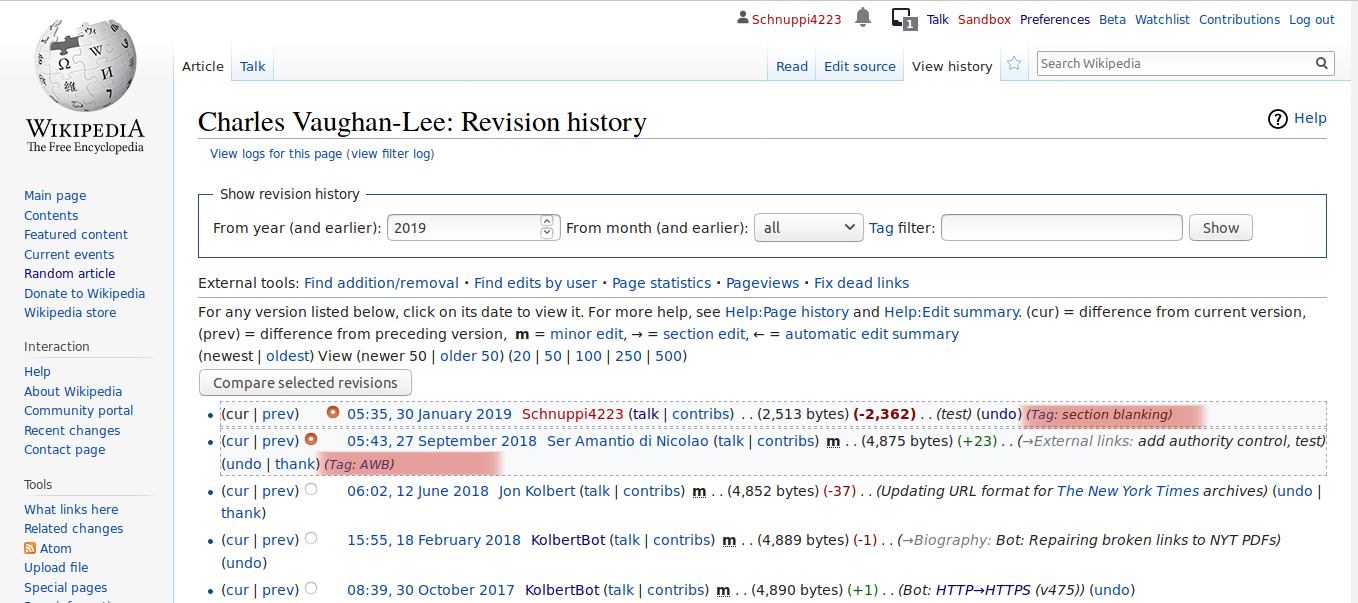
\includegraphics[width=0.9\columnwidth]{pics/screenshots-filter-trigger/Screenshot-tags-in-revision-history.png}
  \caption{Tagged edits are marked as such in a page's revision history}~\label{fig:tags-in-history}
\end{figure}

\begin{figure}
\centering
  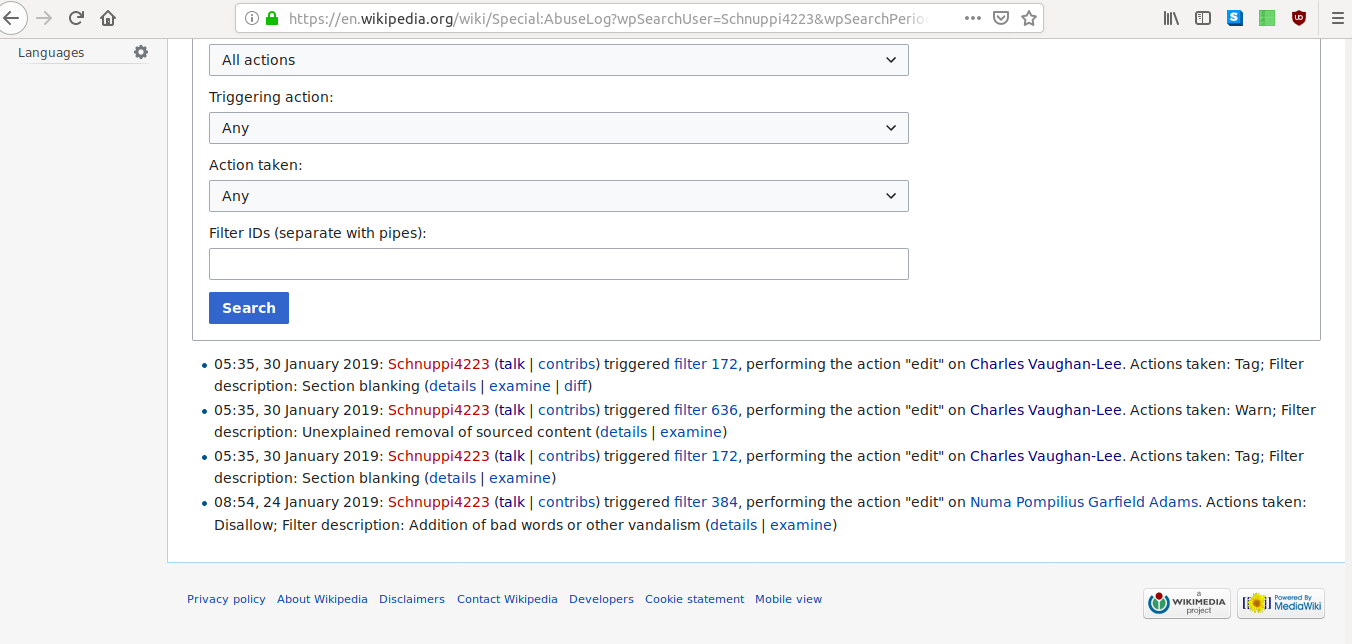
\includegraphics[width=0.9\columnwidth]{pics/screenshots-filter-trigger/Screenshot-abuse-log.png}
  \caption{Abuse Log showing all filter triggers by User Schnuppi4223}~\label{fig:screenshot-abuse-log}
\end{figure}

If the filter is set to disallow, a specific template is shown to the editor: "An automated filter has identified this edit as potentially unconstructive, so it has been disallowed. If this edit is constructive, please report this error. Disruptive editing may result in a block from editing."
"report this error" links to the FalsePositives page: \url{https://en.wikipedia.org/wiki/Wikipedia:Edit_filter/False_positives}
"block from editing" links to \url{https://en.wikipedia.org/wiki/Wikipedia:Blocking_policy}

The edit is not saved.

\begin{figure}
\centering
  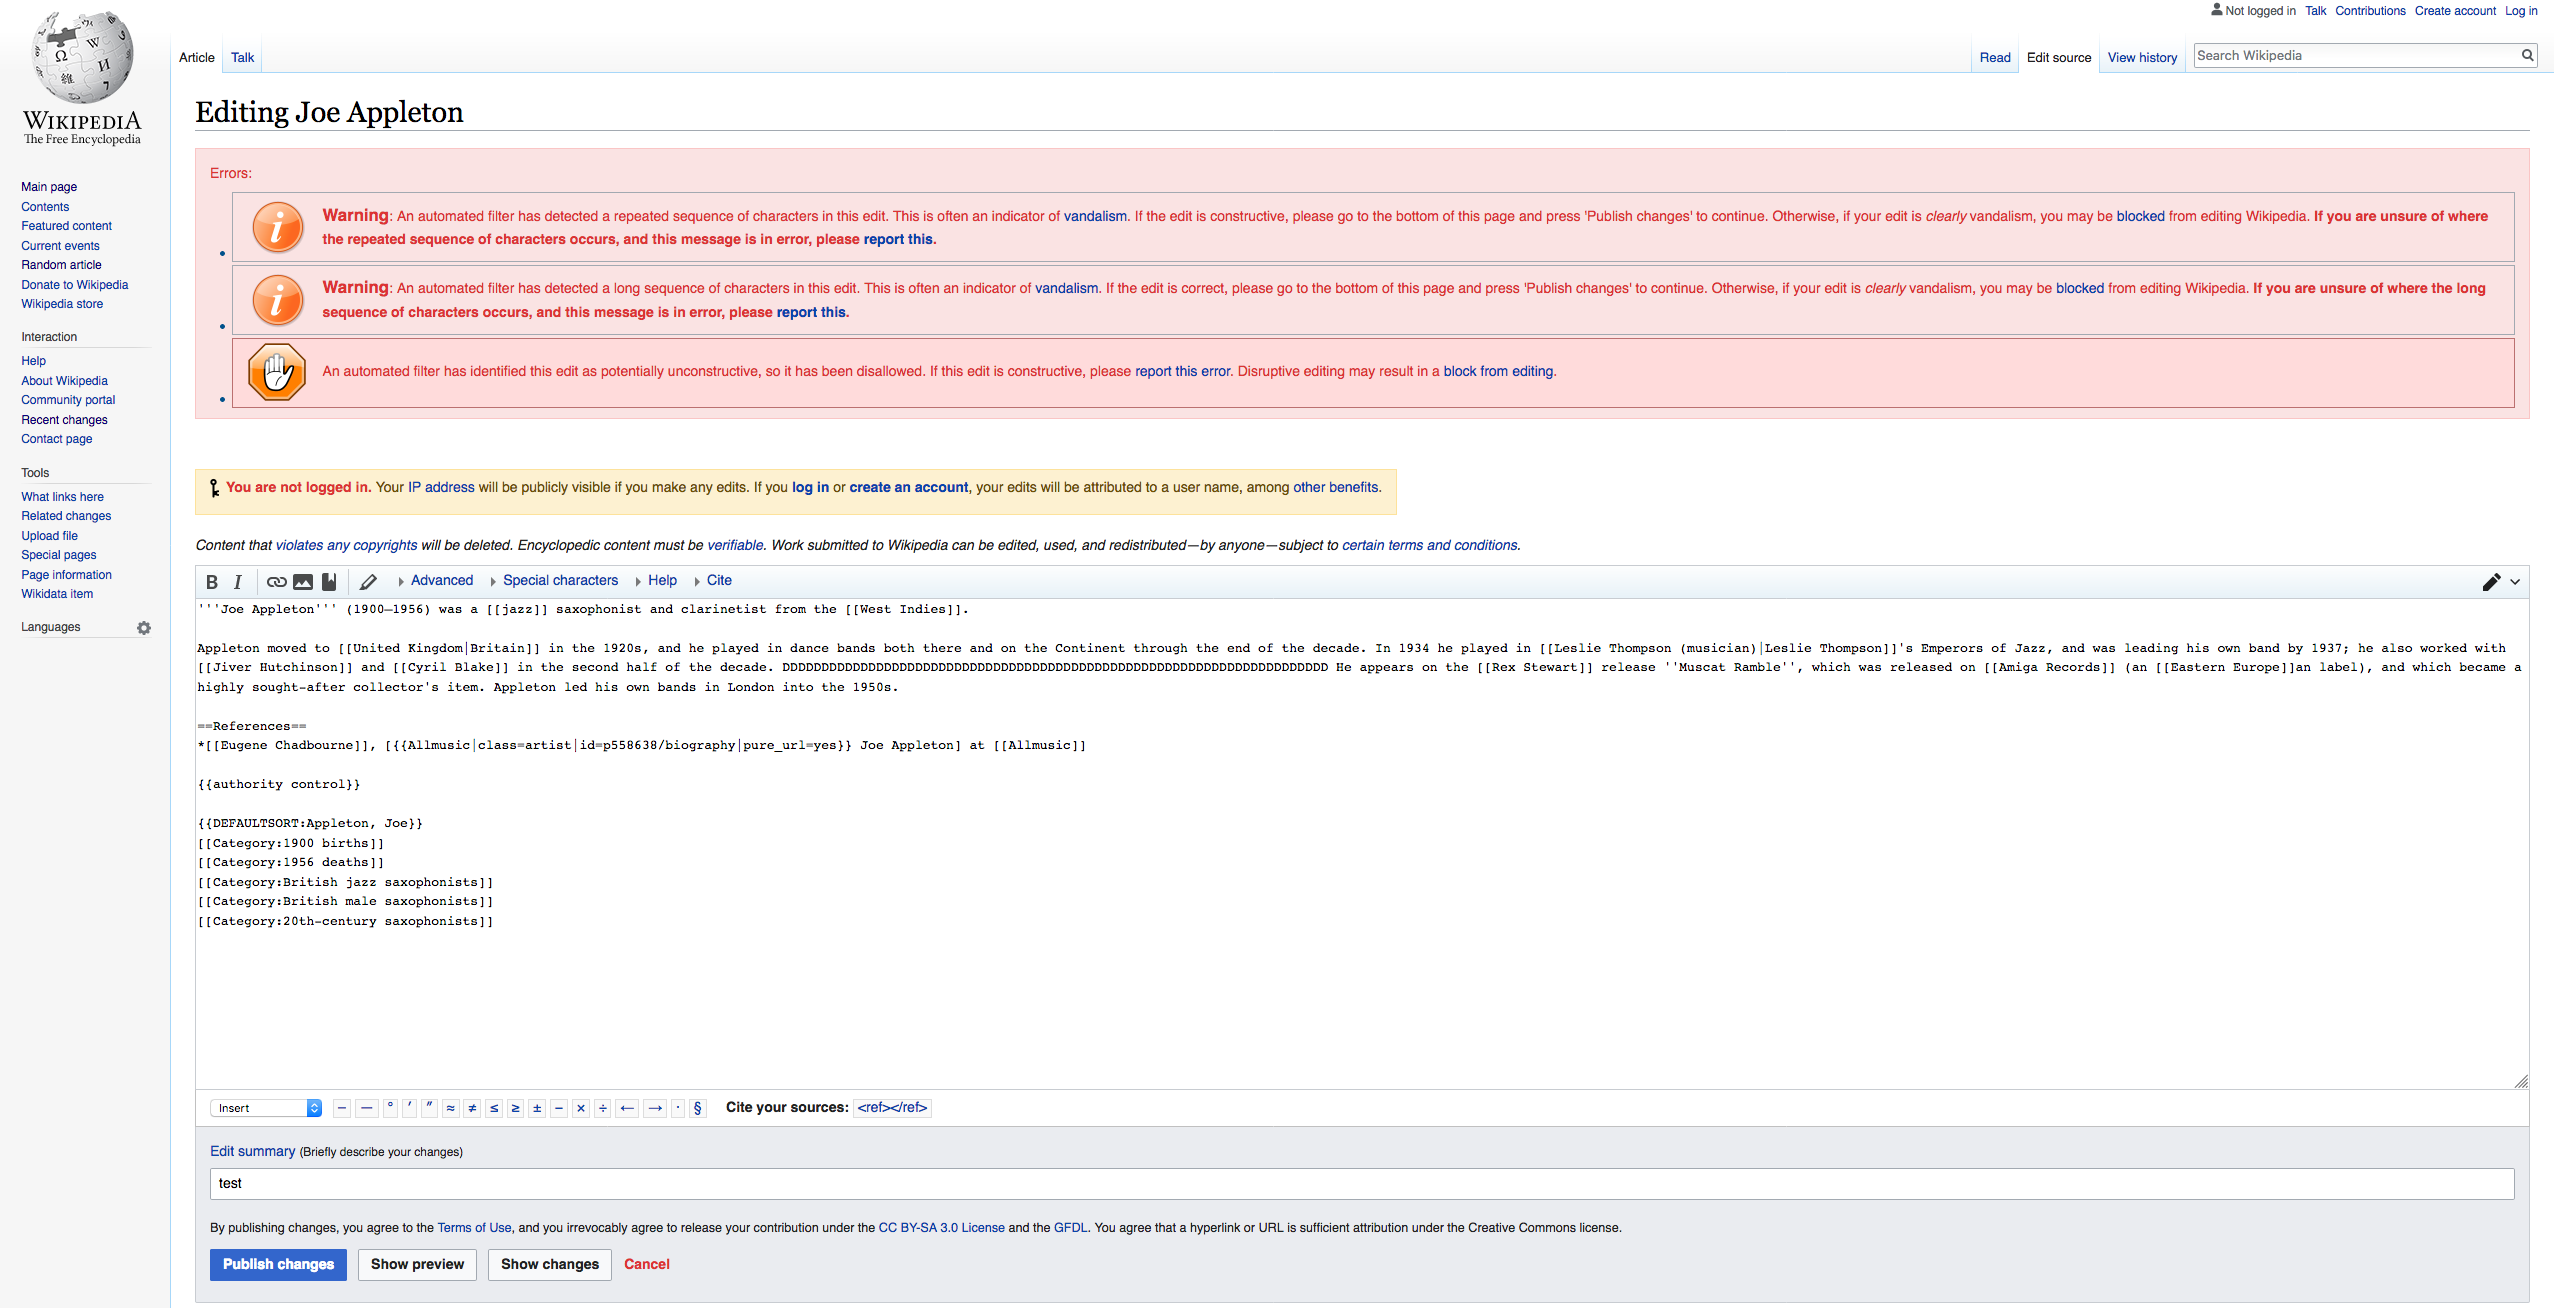
\includegraphics[width=0.9\columnwidth]{pics/screenshots-filter-trigger/Screenshot-trigger-warning-filter.png}
  \caption{Editor gets notified their edit triggered multiple edit filters}~\label{fig:screenshot-warn-disallow}
\end{figure}

\subsection{what happens afterwards}

If a user disagrees with the filter decision, they have the posibility of reporting a false positive
\url{https://en.wikipedia.org/wiki/Wikipedia:Edit_filter/False_positives}

\subsection{How are problems handled?}
%TODO review this part with presi: help to clear up the structure

There are several pages where problematic behaviour concerning edit filters as well as potential solutions are discussed.

For instance, current filters behaviour is discussed on the Edit Filter Noticeboard~\footnote{\url{https://en.wikipedia.org/wiki/Wikipedia:Edit_filter_noticeboard}}.
Issues handled here include changing the edit filter action of single filters, changing edit filter warning templates, problems with specific regexes or variables and proposals for filter deletions.
Furthermore, on the noticeboard discussions take place about giving edit filter manager rights to users, or withdrawing these if a misuse was observed and raising the issue with the editor directly didn't resolve the problem~\cite{Wikipedia:EditFilter}.

False positives among the filter hits are reported and discussed on a separate page~\footnote{\url{https://en.wikipedia.org/wiki/Wikipedia:Edit_filter/False_positives}}.
Edit filter managers monitor this page and improve filters based on true false positives, give advice to good faith editors who tripped a filter or discourage authors of vandalism edits to continue with them.
%TODO who moderates the false positives page? where does the info come from that it is edit filter managers?

Moreover, edit filter managers are advised to consult and comply with personal security best practices (such as choosing a strong password and using two-factor authentication).
If such an account is compromised, it loses its edit filter manager rights and gets blocked, since this threatens site security~\cite{Wikipedia:EditFilter}.

\begin{comment}
\url{https://en.wikipedia.org/wiki/Wikipedia:Edit_filter}
"In the unlikely event that your account is compromised, notify an administrator or bureaucrat (for administrators) immediately so they can block your account and remove any sensitive privileges to prevent damage. "
//interessanterweise is 2factor-auth auch nur für diese speziellen Benutzer*innen erlaubt; sonst kann man die Seite nicht ansehen
\end{comment}


\section{Edit filters' role in the quality control frame}
\subsection{Alternatives}
%TODO: where should this go? Already kind of mentioned in the introducing a filter part

Since edit filters run against every edit saved on Wikipedia, it is generally adviced against rarely tripped filters and a number of alternatives is signaled to edit filter managers and editors proposing new filters.
%TODO: number of filters cannot grow endlessly, every edit is checked against all of them and this consumes computing power! (and apparently haven't been chucked with Moore's law). is this the reason why number of filters has been more or less constanst over the years?
\begin{comment}
\url{https://en.wikipedia.org/wiki/Wikipedia:Edit_filter/Requested}
"Each filter takes time to run, making editing (and to some extent other things) slightly slower. The time is only a few milliseconds per filter, but with enough filters that adds up. When the system is near its limit, adding a new filter may require removing another filter in order to keep the system within its limits."
\end{comment}
For example, there is the page protection mechanism that addresses problems on a single page.
Also, title and spam blacklists exist and these might be the way to handle problems with page titles or link spam~\cite{Wikipedia:EditFilter}.

%************************************************************************

\subsection{Collaboration with bots (and semi-automated tools)}

"There is a bot reporting users tripping certain filters at WP:AIV and WP:UAA; you can specify the filters here."
\url{https://en.wikipedia.org/wiki/User:DatBot/filters}

* consider collaborations filters/bots (e.g. MrZ Bot which puts editors found on the abuse log often on the AIV noticeboard.) are there further exampled for this kind of collaborations?

\url{https://en.wikipedia.org/wiki/Wikipedia:Administrator_intervention_against_vandalism}
\url{https://en.wikipedia.org/wiki/Wikipedia:Bots/Requests_for_approval/Mr.Z-bot_7}

Apparently, Twinkle at least has the possibility of using heuristics from the abuse filter log for its queues.
%TODO check. how about other tools

\begin{comment}
    Not sure where this fits in
\subsection{TOR}
(Interesting side note: editing via TOR is disallowed altogether: "Your IP has been recognised as a TOR exit node. We disallow this to prevent abuse" or similar, check again for wording. Compare: "Users of the Tor anonymity network will show the IP address of a Tor "exit node". Lists of known Tor exit nodes are available from the Tor Project's Tor Bulk Exit List exporting tool." \url{https://en.wikipedia.org/wiki/Wikipedia:Vandalism})
\end{comment}

\section{Fazit}
%Conclusion, resume, bottom line

maybe it's a historical phenomenon (in many regards):
* perhaps there were differences that are not essential anymore, such as:
  * on which infrastructure does it run (part of the core software vs own computers of the bot operators)
  * filters are triggered *before* an edit is even published, whereas bots (and tools) can revert an edit post factum. Is this really an important difference in times when bots need a couple of seconds to revert an edit?
* perhaps the extension was implemented because someone was capable of implementing and working well with this type of systems so they just went and did it (do-ocracy; Wikipedia as a collaborative volunteer project);
* perhaps it still exists in times of fancier machine learning based tools (or bots) because rule-based systems are more transparent/easily understandable for humans and writing a regex is simpler than coding a bot.

%TODO maybe put here the comparison table I've started as a feedback from the status presentation

Question:
Oftentimes edit filter managers are also bot operators; how would they decide when to implement an filter and when a bot?

\begin{comment}
\url{http://www.aaronsw.com/weblog/whorunswikipedia}
"But what’s less well-known is that it’s also the site that anyone can run. The vandals aren’t stopped because someone is in charge of stopping them; it was simply something people started doing. And it’s not just vandalism: a “welcoming committee” says hi to every new user, a “cleanup taskforce” goes around doing factchecking. The site’s rules are made by rough consensus. Even the servers are largely run this way — a group of volunteer sysadmins hang out on IRC, keeping an eye on things. Until quite recently, the Foundation that supposedly runs Wikipedia had no actual employees.
This is so unusual, we don’t even have a word for it. It’s tempting to say “democracy”, but that’s woefully inadequate. Wikipedia doesn’t hold a vote and elect someone to be in charge of vandal-fighting. Indeed, “Wikipedia” doesn’t do anything at all. Someone simply sees that there are vandals to be fought and steps up to do the job."

\end{comment}

\begin{comment}
Can I answer these questions?

* Why are there mechanisms triggered before an edit gets published (such as edit filters), and such triggered afterwards (such as bots)? Is there a qualitative difference?
* I want to help people to do their work better using a technical system (e.g. the edit filters). How can I do this?
* The edit filter system can be embedded in the vandalism prevention frame. Are there other contexts/frames for which it is relevant?

* stick to research questions from Confluence, they are already carefully crafted and narrowed down as appropriate
  Q1 We wanted to improve our understanding of the role of filters in existing algorithmic quality-control mechanisms (bots, ORES, humans).
  Q2 Which type of tasks do these filters take over in comparison to the other mechanisms? How these tasks evolve over time (are they changes in the type, number, etc.)?
  Q3 Since filters are classical rule-based systems, what are suitable areas of application for such rule-based system in contrast to the other ML-based approaches.
\end{comment}
 %Governance, Technic
\chapter{Descriptive overview of Edit Filters on the English Wikipedia}
\label{chap:overview-en-wiki}

\section{Data}

\begin{comment}
vgl \cite{GeiHal2017}
iterative mixed method
combination of:
* quantitative methods: mining big data sets/computational social science
"begin with one or
more large (but often thin) datasets generated by a software platform, which has recorded digital
traces that users leave in interacting on that platform. Such researchers then seek to mine as much
signal and significance from these found datasets as they can at scale in order to answer a research
question"
* more traditional social science/qualitative methods, e.g. interviews, observations, experiments
\end{comment}

The \emph{abuse\_filter} and \emph{abuse\_filter\_action} tables from \emph{enwiki\_p} were downloaded on 6.01.2019 via quarry~\footnote{\url{https://quarry.wmflabs.org/}}.
The complete dataset can be found in the repository for the present paper~\cite{github}. % TODO add a more specific link

These tables, along with \emph{abuse\_filter\_log} and \emph{abuse\_filter\_history}, are created and used by the AbuseFilter MediaWiki extension~\cite{gerrit-abusefilter}.
Selected queries have been run against the \emph{abuse\_filter\_log} table as well.
Unfortunately, currently the \emph{abuse\_filter\_history} table is not exposed to the public due to security/privacy concerns~\cite{phabricator}.
We hope to be shortly able to access a view of this table in order to conduct historic inquirements.

The schemas of these tables can be viewed in Figures~\ref{fig:db-schemas-af},~\ref{fig:db-schemas-afl},~\ref{fig:db-schemas-afh} and~\ref{fig:db-schemas-afa}.

\begin{figure*}
\begin{verbatim}
abuse_filter
+--------------------+---------------------+------+-----+---------+----------------+
| Field              | Type                | Null | Key | Default | Extra          |
+--------------------+---------------------+------+-----+---------+----------------+
| af_id              | bigint(20) unsigned | NO   | PRI | NULL    | auto_increment |
| af_pattern         | blob                | NO   |     | NULL    |                |
| af_user            | bigint(20) unsigned | NO   | MUL | NULL    |                |
| af_user_text       | varbinary(255)      | NO   |     | NULL    |                |
| af_timestamp       | binary(14)          | NO   |     | NULL    |                |
| af_enabled         | tinyint(1)          | NO   |     | 1       |                |
| af_comments        | blob                | YES  |     | NULL    |                |
| af_public_comments | tinyblob            | YES  |     | NULL    |                |
| af_hidden          | tinyint(1)          | NO   |     | 0       |                |
| af_hit_count       | bigint(20)          | NO   |     | 0       |                |
| af_throttled       | tinyint(1)          | NO   |     | 0       |                |
| af_deleted         | tinyint(1)          | NO   |     | 0       |                |
| af_actions         | varbinary(255)      | NO   |     |         |                |
| af_global          | tinyint(1)          | NO   |     | 0       |                |
| af_group           | varbinary(64)       | NO   | MUL | default |                |
+--------------------+---------------------+------+-----+---------+----------------+
\end{verbatim}
  \caption{abuse\_filter schema}~\label{fig:db-schemas-af}
\end{figure*}

\begin{figure*}
\begin{verbatim}
abuse_filter_log
+------------------+---------------------+------+-----+---------+----------------+
| Field            | Type                | Null | Key | Default | Extra          |
+------------------+---------------------+------+-----+---------+----------------+
| afl_id           | bigint(20) unsigned | NO   | PRI | NULL    | auto_increment |
| afl_filter       | varbinary(64)       | NO   | MUL | NULL    |                |
| afl_user         | bigint(20) unsigned | NO   | MUL | NULL    |                |
| afl_user_text    | varbinary(255)      | NO   |     | NULL    |                |
| afl_ip           | varbinary(255)      | NO   | MUL | NULL    |                |
| afl_action       | varbinary(255)      | NO   |     | NULL    |                |
| afl_actions      | varbinary(255)      | NO   |     | NULL    |                |
| afl_var_dump     | blob                | NO   |     | NULL    |                |
| afl_timestamp    | binary(14)          | NO   | MUL | NULL    |                |
| afl_namespace    | tinyint(4)          | NO   | MUL | NULL    |                |
| afl_title        | varbinary(255)      | NO   |     | NULL    |                |
| afl_wiki         | varbinary(64)       | YES  | MUL | NULL    |                |
| afl_deleted      | tinyint(1)          | NO   |     | 0       |                |
| afl_patrolled_by | int(10) unsigned    | YES  |     | NULL    |                |
| afl_rev_id       | int(10) unsigned    | YES  | MUL | NULL    |                |
| afl_log_id       | int(10) unsigned    | YES  | MUL | NULL    |                |
+------------------+---------------------+------+-----+---------+----------------+
\end{verbatim}
  \caption{abuse\_filter\_log schema}~\label{fig:db-schemas-afl}
\end{figure*}

\begin{figure*}
\begin{verbatim}
abuse_filter_history
+---------------------+---------------------+------+-----+---------+----------------+
| Field               | Type                | Null | Key | Default | Extra          |
+---------------------+---------------------+------+-----+---------+----------------+
| afh_id              | bigint(20) unsigned | NO   | PRI | NULL    | auto_increment |
| afh_filter          | bigint(20) unsigned | NO   | MUL | NULL    |                |
| afh_user            | bigint(20) unsigned | NO   | MUL | NULL    |                |
| afh_user_text       | varbinary(255)      | NO   | MUL | NULL    |                |
| afh_timestamp       | binary(14)          | NO   | MUL | NULL    |                |
| afh_pattern         | blob                | NO   |     | NULL    |                |
| afh_comments        | blob                | NO   |     | NULL    |                |
| afh_flags           | tinyblob            | NO   |     | NULL    |                |
| afh_public_comments | tinyblob            | YES  |     | NULL    |                |
| afh_actions         | blob                | YES  |     | NULL    |                |
| afh_deleted         | tinyint(1)          | NO   |     | 0       |                |
| afh_changed_fields  | varbinary(255)      | NO   |     |         |                |
| afh_group           | varbinary(64)       | YES  |     | NULL    |                |
+---------------------+---------------------+------+-----+---------+----------------+
\end{verbatim}
  \caption{abuse\_filter\_history schema}~\label{fig:db-schemas-afh}
\end{figure*}

\begin{figure*}
\begin{verbatim}
abuse_filter_action
+-----------------+---------------------+------+-----+---------+-------+
| Field           | Type                | Null | Key | Default | Extra |
+-----------------+---------------------+------+-----+---------+-------+
| afa_filter      | bigint(20) unsigned | NO   | PRI | NULL    |       |
| afa_consequence | varbinary(255)      | NO   | PRI | NULL    |       |
| afa_parameters  | tinyblob            | NO   |     | NULL    |       |
+-----------------+---------------------+------+-----+---------+-------+
\end{verbatim}
  \caption{abuse\_filter\_action schema}~\label{fig:db-schemas-afa}
\end{figure*}


\textbf{Interesting questions}
\begin{itemize}
    \item how many filters are there (were there over the years): 954 filters (stand: 06.01.2019); TODO: historically?; This includes deleted filters
    \item what do the most active filters do?: see~\ref{tab:most-active-actions}
    \item get a sense of what gets filtered (more qualitative): TODO: refine after sorting through manual categories; preliminary: vandalism; unintentional suboptimal behavior from new users who don't know better ("good faith edits") such as blanking an article/section; creating an article without categories; adding larger texts without references; large unwikified new article (180); or from users who are too lazy (to write proper edit summaries; editing behaviours and styles not suitable for an encyclopedia (poor grammar/not commiting to orthography norms; use of emoticons and !; ascii art?); "unexplained removal of sourced content" (636) may be an attempt to silence a view point the editor doesn't like; self-promotion(adding unreferenced material to BLP; "users creating autobiographies" 148;); harassment; sockpuppetry; potential copyright violations; that's more or less it actually. There's a third bigger cluster of maintenance stuff, such as tracking bugs or other problems, trying to sort through bot edits and such. For further details see the jupyter notebook.
        Interestingly, there was a guideline somewhere stating that no trivial formatting mistakes should trip filters\cite{Wikipedia:EditFilterRequested}
        %TODO (what exactly are trivial formatting mistakes? starting every paragraph with a small letter; or is this orthography and trivial formatting mistakes references only Wiki syntax? I think though they are similar in scale and impact)
        I actually think, a bot fixing this would be more appropriate.
    \item has the willingness of the community to use filters increased over time?: looking at aggregated values of number of triggered filters per year, the answer is rather it's quite constant; TODO: plot it at a finer granularity
        when aggregating filter triggers per month, one notices that there's an overall slight upward tendency.
        Also, there is a dip in the middle of 2014 and a notable peak at the beginning of 2016, that should be investigated further.
    \item how often were (which) filters triggered: see \url{filter-lists/20190106115600_filters-sorted-by-hits.csv} and~\ref{tab:most-active-actions}; see also jupyter notebook for aggregated hitcounts over tagged categories
    \item percentage of triggered filters/all edits; break down triggered filters according to typology: TODO still need the complete abuse\_filter\_log table!; and probably further dumps in order to know total number of edits
    \item percentage filters of different types over the years: according to actions (I need a complete abuse\_filter\_log table for this!); according to self-assigned tags %TODO plot!
\end{itemize}

\textbf{Questions on abuse\_filter table}
\begin{itemize}
    \item how many filters are there altogether
    \item how many are enabled/disabled?
    \item how many hidden filters? how many of them are enabled
    \item how many are marked as deleted? (how many of them are hidden?)
    \item how many global? (what does global mean?)
    \item how many throttled? (what does this mean?)
    \item how many currently trigger which action (disallow, warn, throttle, tag, ..)?
    \item explore timestamp (I think it means "last modified"): have a lot of filters been modified recently?
    \item what are the values in the "group" column? what do they mean?
    \item which are the most frequently triggered filters of all time? \ref{tab:most-active-actions}
    \item is it new filters that get triggered most frequently? or are there also very active old ones? -- we have the most active filters per year, where we can observe this. It's a mixture of older and newer filter IDs (they get an incremental ID, so it is somewhat obvious what's older and what's newer); is there a tendency to split and refine older filters?
    \item how many different edit filter editors are there (af\_user)?
    \item categorise filters according to which name spaces they apply to; pay special attention to edits in user/talks name spaces (may be indication of filtering harassment)
\end{itemize}

\textbf{Questions on abuse\_filter\_log table}
\begin{itemize}
    \item how often were filters with different actions triggered? (afl\_actions)
    \item what types of users trigger the filters (IPs? registered?) : IPs: 16,489,266, logged in users: 6,984,897 (Stand 15.03.2019);
    \item on what articles filters get triggered most frequently (afl\_title)
    \item what types of user actions trigger filters most frequently? (afl\_action) (edit, delete, createaccount, move, upload, autocreateaccount, stashupload)
    \item in which namespaces get filters triggered most frequently?
\end{itemize}

\textbf{Questions on abuse\_filter\_action table}
\begin{itemize}
    \item how many filters trigger any particular action (at the moment)?
    \item how many different parameters are there (i.e. tags when tagging, or templates to show upon a warning)?
\end{itemize}

\textbf{Number of unique filters that were triggered each year since 2009:}
owing to quarries we have all the filters that were triggered from the filter log per year, from 2009 (when filters were first introduced/the MediaWiki extension was enabled) till end of 2018 with their corresponding number of times being triggered:
\begin{table}
  \centering
  \begin{tabular}{l r }
    % \toprule
    Year & Num of distinct filters \\
    \hline
    2009 & 220 \\
    2010 & 163 \\
    2011 & 161 \\
    2012 & 170 \\
    2013 & 178 \\
    2014 & 154 \\
    2015 & 200 \\
    2016 & 204 \\
    2017 & 231 \\
    2018 & 254 \\
    % \bottomrule
  \end{tabular}
  \caption{Count of distinct filters that got triggered each year}~\label{tab:active-filters-count}
\end{table}

data is still not enough for us to talk about a tendency towards introducing more filters (after the initial dip)

%TODO: number of filters cannot grow endlessly, every edit is checked against all of them and this consumes computing power! (and apparently haven't been chucked with Moore's law). is this the reason why number of filters has been more or less constanst over the years?
\begin{comment}
\url{https://en.wikipedia.org/wiki/Wikipedia:Edit_filter/Requested}
"Each filter takes time to run, making editing (and to some extent other things) slightly slower. The time is only a few milliseconds per filter, but with enough filters that adds up. When the system is near its limit, adding a new filter may require removing another filter in order to keep the system within its limits."
\end{comment}

\textbf{Most frequently triggered filters for each year:}
10 most active filters per year:
\begin{table}
  \centering
  \begin{tabular}{r r }
    % \toprule
    Filter ID & Publicly available description & Hitcount \\ %TODO is the hitcount for the year or altogether till now?
    \hline
    135 & repeating characters & 175455 \\
    30 & "large deletion from article by new editors" & 160302 \\
    61 & "new user removing references" ("new user" is handled by "!("confirmed" in user\_groups)") & 147377 \\
    18 & Test type edits from clicking on edit bar & 133640 \\
    3 & "new user blanking articles" & 95916 \\
    172 & "section blanking" & 89710 \\
    50 & "shouting" (contribution consists of all caps, numbers and punctuation) & 88827 \\
    98 & "creating very short new article" & 80434 \\
    65 & "excessive whitespace" (note: "associated with ascii art and some types of vandalism") & 74098 \\
    132 & "removal of all categories" & 68607 \\
    % \bottomrule
  \end{tabular}
  \caption{10 most active filters in 2009}~\label{tab:most-active-2009}
\end{table}

\begin{table}
  \centering
  \begin{tabular}{r r }
    % \toprule
    Filter ID & Publicly available description & Hitcount \\
    \hline
    61 & "new user removing references" ("new user" is handled by "!("confirmed" in user\_groups)") & 245179 \\
    135 & repeating characters & 242018 \\
    172 & "section blanking" & 148053 \\
    30 & "large deletion from article by new editors" & 119226 \\
    225 & Vandalism in all caps & 109912 \\
    3 & "new user blanking articles" & 105376 \\
    50 & "shouting" (contribution consists of all caps, numbers and punctuation) & 101542 \\
    132 & "removal of all categories" & 78633 \\
    189 & BLP vandalism or libel & 74528 \\
    98 & "creating very short new article" & 54805 \\
    % \bottomrule
  \end{tabular}
  \caption{10 most active filters in 2010}~\label{tab:most-active-2010}
\end{table}

\begin{table}
  \centering
  \begin{tabular}{r r }
    % \toprule
    Filter ID & Publicly available description & Hitcount \\
    \hline
    61 & "new user removing references" ("new user" is handled by "!("confirmed" in user\_groups)") & 218493 \\
    135 & repeating characters & 185304 \\
    172 & "section blanking" & 119532 \\
    402 & New article without references & 109347 \\
    30 & Large deletion from article by new editors & 89151 \\
    3 & "new user blanking articles" & 75761 \\
    384 & Addition of bad words or other vandalism & 71911 \\
    225 & Vandalism in all caps & 68318 \\
    50 & "shouting" (contribution consists of all caps, numbers and punctuation) & 67425 \\
    432 & Starting new line with lowercase letters & 66480 \\
    % \bottomrule
  \end{tabular}
  \caption{10 most active filters in 2011}~\label{tab:most-active-2011}
\end{table}

\begin{table}
  \centering
  \begin{tabular}{r r }
    % \toprule
    Filter ID & Publicly available description & Hitcount \\
    \hline
    135 & repeating characters & 173830 \\
    384 & Addition of bad words or other vandalism & 144202 \\
    432 & Starting new line with lowercase letters & 126156 \\
    172 & "section blanking" & 105082 \\
    30 & Large deletion from article by new editors & 93718 \\
    3 & "new user blanking articles" & 90724 \\
    380 & Multiple obscenities & 67814 \\
    351 & Text added after categories and interwiki & 59226 \\
    279 & Repeated attempts to vandalize & 58853 \\
    225 & Vandalism in all caps & 58352 \\
    % \bottomrule
  \end{tabular}
  \caption{10 most active filters in 2012}~\label{tab:most-active-2012}
\end{table}

\begin{table}
  \centering
  \begin{tabular}{r r }
    % \toprule
    Filter ID & Publicly available description & Hitcount \\
    \hline
    135 & repeating characters & 133309 \\
    384 & Addition of bad words or other vandalism & 129807 \\
    432 & Starting new line with lowercase letters & 94017 \\
    172 & "section blanking" & 92871 \\
    30 & Large deletion from article by new editors & 85722 \\
    279 & Repeated attempts to vandalize & 76738 \\
    3 & "new user blanking articles" & 70067 \\
    380 & Multiple obscenities & 58668 \\
    491 & Edits ending with emoticons or ! & 55454 \\
    225 & Vandalism in all caps & 48390 \\
    % \bottomrule
  \end{tabular}
  \caption{10 most active filters in 2013}~\label{tab:most-active-2013}
\end{table}

\begin{table}
  \centering
  \begin{tabular}{r r }
    % \toprule
    Filter ID & Publicly available description & Hitcount \\
    \hline
    384 & Addition of bad words or other vandalism & 111570 \\
    135 & repeating characters & 111173 \\
    279 & Repeated attempts to vandalize & 97204 \\
    172 & "section blanking" & 82042 \\
    432 & Starting new line with lowercase letters & 75839 \\
    30  & Large deletion from article by new editors & 62495 \\
    3 & "new user blanking articles" & 60656 \\
    636 & Unexplained removal of sourced content & 52639 \\
    231 & Long string of characters containing no spaces & 39693 \\
    380 & Multiple obscenities & 39624 \\
    % \bottomrule
  \end{tabular}
  \caption{10 most active filters in 2014}~\label{tab:most-active-2014}
\end{table}

\begin{table}
  \centering
  \begin{tabular}{r r }
    % \toprule
    Filter ID & Publicly available description & Hitcount \\
    \hline
    650 & Creation of a new article without any categories & 226460 \\
    61 & New user removing references & 196986 \\
    636 & Unexplained removal of sourced content & 191320 \\
    527 & T34234: log/throttle possible sleeper account creations & 189911 \\
    633 & Possible canned edit summary & 162319 \\
    384 & Addition of bad words or other vandalism & 141534 \\
    279 & Repeated attempts to vandalize & 110137 \\
    135 & repeating characters & 99057 \\
    686 & IP adding possibly unreferenced material to BLP & 95356 \\
    172 & "section blanking" & 82874 \\
    % \bottomrule
  \end{tabular}
  \caption{10 most active filters in 2015}~\label{tab:most-active-2015}
\end{table}

\begin{table}
  \centering
  \begin{tabular}{r r }
    % \toprule
    Filter ID & Publicly available description & Hitcount \\
    \hline
    527 & T34234: log/throttle possible sleeper account creations & 437099 \\
    61 & New user removing references & 274945 \\
    650 & Creation of a new article without any categories & 229083 \\
    633 & Possible canned edit summary & 218696 \\
    636 & Unexplained removal of sourced content & 179948 \\
    384 & Addition of bad words or other vandalism & 179871 \\
    279 & Repeated attempts to vandalize & 106699 \\
    135 & repeating characters & 95131 \\
    172 & "section blanking" & 79843 \\
    30 & Large deletion from article by new editors & 68968 \\
    % \bottomrule
  \end{tabular}
  \caption{10 most active filters in 2016}~\label{tab:most-active-2016}
\end{table}

\begin{table}
  \centering
  \begin{tabular}{r r }
    % \toprule
    Filter ID & Publicly available description & Hitcount \\
    \hline
    61 & New user removing references & 250394 \\
    633 & Possible canned edit summary & 218146 \\
    384 & Addition of bad words or other vandalism & 200748 \\
    527 & T34234: log/throttle possible sleeper account creations & 192441 \\
    636 & Unexplained removal of sourced content & 156409 \\
    650 & Creation of a new article without any categories & 151604 \\
    135 & repeating characters & 80056 \\
    172 & "section blanking" & 70837 \\
    712 & Possibly changing date of birth in infobox & 59537 \\
    833 & Newer user possibly adding unreferenced or improperly referenced material & 58133 \\
    % \bottomrule
  \end{tabular}
  \caption{10 most active filters in 2017}~\label{tab:most-active-2017}
\end{table}

\begin{table}
  \centering
  \begin{tabular}{r r }
    % \toprule
    Filter ID & Publicly available description & Hitcount \\
    \hline
    527 & T34234: log/throttle possible sleeper account creations & 358210 \\
    61 & New user removing references & 234867 \\
    633 & Possible canned edit summary & 201400 \\
    384 & Addition of bad words or other vandalism & 177543 \\
    833 & Newer user possibly adding unreferenced or improperly referenced material & 161030 \\
    636 & Unexplained removal of sourced content & 144674 \\
    650 & Creation of a new article without any categories & 79381 \\
    135 & repeating characters & 75348 \\
    686 & IP adding possibly unreferenced material to BLP & 70550 \\
    172 & "section blanking" & 64266 \\
    % \bottomrule
  \end{tabular}
  \caption{10 most active filters in 2018}~\label{tab:most-active-2018}
\end{table}

\textbf{what do the most active filters do?}

\begin{table*}
  \centering
    \begin{tabular}{r p{10cm} p{5cm} }
    % \toprule
    Filter ID & Publicly available description & Actions \\ %TODO maybe add hitcount?
    \hline
      135 & repeating characters & tag, warn \\
      30 & "large deletion from article by new editors" & tag, warn \\
      61 & "new user removing references" ("new user" is handled by "!("confirmed" in user\_groups)") & tag \\
      18 & "test type edits from clicking on edit bar" (people don't replace Example texts when click-editing) & deleted in Feb 2012 \\
      3 & "new user blanking articles" & tag, warn \\
      172 & "section blanking" & tag \\
      50 & "shouting" (contribution consists of all caps, numbers and punctuation) & tag, warn \\
      98 & "creating very short new article" & tag \\
      65 & "excessive whitespace" (note: "associated with ascii art and some types of vandalism") & deleted in Jan 2010 \\
      132 & "removal of all categories" & tag, warn \\
      225 & "vandalism in all caps" (difference to 50? seems to be swear words, but shouldn't they be catched by 50 anyway?) & disallow \\
      189 & "BLP vandalism or libel" & tag \\
      402 & "new article without references" & deleted in Apr 2013, before that disabled with comment "disabling, no real use" \\
      384 & "addition of bad words or other vandalism" (seems to be a blacklist) & disallow \\
      432 & "starting new line with lower case letters" & tag, warn //I recall there was a rule of thumb recommending not to user filters for style things? although that's not really style, but rather wrong grammar.. \\
      380 & hidden; public comment "multiple obscenities" & disallow \\
      351 & "text added after categories and interwiki" & tag, warn \\
      279 & "repeated attempts to vandalise" & tag, throttle (triggered when someone hits "edit" repeatedly in a short ammount of time) \\
      491 & "edits ending with emoticons or !" & tag, warn \\
      636 & "unexplained removal of sourced content" & warn (that, together with 634 and 635 refutes my theory that warn always goes together with tag) \\
      231 & "long string of characters containing no spaces" (that's surely english though^^) & tag, warn \\
      650 & "creation of a new article without any categories" & (log only) \\
      527 & hidden; public comments "T34234: log/throttle possible sleeper account creations" & throttle \\
      633 & "possible canned edit summary" (apparently pre-filled on mobile though) & tag \\
      686 & "IP adding possible unreferenced material to BLP" (BLP= biography of living people? I thought, it was forbidden to edit them without a registered account) & (log only) \\
      712 & "possibly changing date of birth in infobox" ("possibly"? and I thought infoboxes were pre-generated from wikidata?) & (log only) \\
      833 & "newer user possibly adding a unreferenced or improperly referenced material" & (log only) \\
  \end{tabular}
  \caption{What do most active filters do?}~\label{tab:most-active-actions}
\end{table*}

A lot of filters are disabled/deleted bc:
* they hit too many false positives
* they were implemented to target specific incidents and these vandalism attempts stopped
* they were tested and merged into other filters
* there were too few hits and the conditions were too expensive

Multiple filters have the comment "let's see whether this hits something", which brings us to the conclusion that edit filter editors have the right and do implement filters they consider necessary


%\subsection{Types of edit filters}
%We can sort filters into categories along various criteria.
%For now we don't have a different criteria...

\section{Patterns in filters creation and usage}
* What are typical filter usage patterns?
  ** switched on for a while, then deactivated and never activated again?: 81 (bad charts), 167 (two brief disables underway), 302 (switched off on the grounds of insufficient activity)
     ** switched on for a short while and then powered down: mostly stuff merged to other filters; or for which the community decides filter is not an appropriate solution (308); or decides to not implement the thing (that way); 290 (disabled, since relevant pages were protected)
     ** or switched off after a short while because there were no hits: 304, 67, 122
     ** or switched off after a longer while, because it was not tripped frequently, in order to save conditions from the condition limit: 211 ("Disable, appears to be inactive (log only filter). If you are using this filter, please let me know, and I'll reenable it -Prodego")
     ** switched off bc merged to another filter 440 was merged in 345
     ** on for a short while and off again bc?? (false positives is a plausible option here): 394
  ** switched on and still on: 11 (verify), 79 (with brief periods of being disabled for couple of minutes/hours, probably in order to update the pattern), 164, 642 (if we ignore the 2min period it was disabled on 13.4.2018), 733 (2.11.2015-present), 29 (18.3.2009-present), 30 (18.3.2009-present), 33 (18.3.2009-present), 39 (18.3.2009-present), 50 (18.3.2009-present), 59 (19.3.2009-present), 80 (22.3.2009-present)
  ** switched on for a while, deactivated for a while, activated again?: 61, 98 (was deactivated briefly since an editor found the "warn" action unfounded; re-enabled to tag), 148 ("20160213 - disabled - possible technical issue - see edit filter noticeboard - xaosflux")
  ** switched on and stayed on, with the exception of brief periods of time when the filter was deactivated (and the activated again), probably in order to update the conditions: 79, 135 (there were couple of others in Shirik's list, go back and look);
  ** irregular?

* What do filters target: general behaviour vs edits by single users
  ** there are quite some filters targeting particular users: 290 (targets an IP range)
  ** there are also some targetting particular pages (verify!), although this clashed with the guidelines
  ** and there are some filtering in general
  ** there are also filters such as 199 (Unflagged bots) which were implemented in order to track something which was not quite malicious or abusive and were thus deemed inappropriate use of filters by the community and consequently (quite swiftly) deleted
  ** some target insults in general and some contain regexes containing very specifically insults directed towards edit filter managers (see filter 12)

* How do filters emerge?
  ** an older filter is split? 79 was split out of 61, apparently; 285 is split between "380, 384, 614 and others"; 174 is split from 29
  ** several older filters are merged?
  ** or functionality of an older filter is took and extended in a newer one (479->631); (82->278); (358->633);
  ** new condition(s) are tested and then merged into existing filter : stuff from 292 was merged to 135 (https://en.wikipedia.org/wiki/Special:AbuseFilter/history/135/diff/prev/4408 , also from 366; following the comments from https://en.wikipedia.org/wiki/Special:AbuseFilter/292 it was not conceived as a test filter though, but it was rather merged in 135 post-factum to save conditions); 440 was merged into 345; apparently 912 was merged into 11 (but 11 still looks like checking for "they suck" only^^)
  ** an incident caught repeatedly by a filter motivates the creation of a dedicated filter (994)
  ** filter is shut down, because editors notice there are 2 (or more filters) that do nearly identical checks: 344 shut down because of 3

  ** "in addition to filter 148, let's see what we get - Cen" (https://en.wikipedia.org/wiki/Special:AbuseFilter/188) // this illustrates the point that edit filter managers do introduce stuff they feel like introducing just to see if it catches something

* How stable is the filter maker community?
  ** how many new users have become part of it over time?
  ** Has it been the same people from the very beginning?
  ** are there a couple of very active edit filter managers, that are also (informal) leaders?
  ** Do edit filter managers specialize on particular types of filters (e.g. vandalism vs good faith?)

* How are filter actions set
  ** there's this pattern that all actions but logging (which cannot be switched off) are took out, when edit filter managers are updating the regex of the filter
  ** there's a tendency of editors to hide filters just for the heck of it (at least there are never clear reasons given), which is then reverted by other editors with the comment that it is not needed: 148, 225 (consesus that general vandalism filters should be public [Special:Permalink/784131724#Privacy of general vandalism filters), 260 (similar to 225), 285 (same), 12 (same), 39 (unhidden with the comment "made filter public again - these edits are generally made by really unsophisticated editors who barely know how to edit a page. --zzuuzz")
  ** oftentimes, when a hidden filter is marked as "deleted" it is made public

\section{Public and Hidden Filters}

The first noticeable typology is along the line public/private filters.

It is calling attention that nearly 2/3 of all edit filters are not viewable by the general public.
%TODO: remark that it was to investigate this historically; or is there still an easy way to do this?

The guidelines call for hiding filters ``only where necessary, such as in long-term abuse cases where the targeted user(s) could review a public filter and use that knowledge to circumvent it.''~\cite{Wikipedia:EditFilter}.
Further, they suggest caution in filter naming and giving just simple description of the overall disruptive behaviour rather than naming specificuser that is causing the disruptions.
(The later is not always complied with, there are indeed filters named after the accounts causing a disruption.)

Only edit filter editors (who have the \emph{abusefilter-modify} permission) and editors with the \emph{abusefilter-view-private} permission can view hidden filters.
The later is given to edit filter helpers - editors interested in helping with edit filters who still do not meet certain criteria in order to be granted the full \emph{abusefilter-modify} permission, editors working with edit filters on other wikis interested in learning from the filter system on English Wikipedia, and Sockpuppet investigation clerks~\cite{Wikipedia:EditFilterHelper}.
As of March 17, 2019, there are 16 edit filter helpers on EN Wikipedia~\footnote{\url{https://en.wikipedia.org/wiki/Special:ListUsers/abusefilter-helper}}.
Also, all administrators are able to view hidden filters.

There is also a designated mailing list for discussing these: wikipedia-en-editfilters@lists.wikimedia.org.
It is specifically indicated that this is the communication channel to be used when dealing with harassment (by means of edit filters)~\cite{Wikipedia:EditFilter}.
It is signaled, that the mailing list is meant for sensitive cases only and all general discussions should be held on-wiki~\cite{Wikipedia:EditFilter}.

\begin{comment}
\url{https://en.wikipedia.org/wiki/Wikipedia:Edit_filter}
"Non-admins in good standing who wish to review a proposed but hidden filter may message the mailing list for details."
// what is "good standing"?
// what are the arguments for hiding a filter? --> particularly obnoctious vandals can see how their edits are being filtered and circumvent them; security through obscurity -- compare also comments on the TalkPage; this is not crypto.
// are users still informed if their edit triggers a hidden filter? - most certainly; the warnings logic has nothing to do with whether the filter is hidden or not

"For all filters, including those hidden from public view, a brief description of what the rule targets is displayed in the log, the list of active filters, and in any error messages generated by the filter. " //yeah, well, that's the public comment, aka name of the filter

"Be careful not to test sensitive parts of private filters in a public test filter (such as Filter 1): use a private test filter (for example Filter 2) if testing is required."

\end{comment}

\section{Types of edit filters: Manual Classification}

Apart from filter typologies that can be derived directly from the DB schema (available fields/existing features), we propose a manual classification of the types of edits edit filters found on the EN Wikipedia target (there are edit filters with different purposes).

Based on the GT methodology, I scrutinised all filters, with their patterns, comments and actions. %TODO define more precisely what exactly are we studying
We found 3 big clusters of filters that we labeled ``vandalism'', ``good faith'' and ``maintenance''.
It was not always a straightforward decision to determine what type of edits a certain filter is targeting.
This was of course, particularly challenging for private filters where only the public comment (name) of the filter was there to guide us.
On the other hand, guidelines state up-front that filters should be hidden only in cases of particularly persistent vandalism, in so far it is probably safe to establish that all hidden filters target some type of vandalism.
However, the classification was difficult for public filters as well, since oftentimes what makes the difference between a good-faith and a vandalism edit is not the content of the edit but the intention of the editor.
While there are cases of juvenile vandalism (putting random swear words in articles) or characters repetiton vandalism which are pretty obvious, that is not the case for sections or articles blanking for example. %TODO explain why
In such ambiguous cases, we can be guided by the action the filter triggers (if it is ``disallow'' the filter is most probably targeting vandalism).
At the end, we labeled most ambiguous cases with both ``vandalism'' and ``good faith''.

In the subsections that follow we discuss the salient properties of each manually labeled category.


Following filter categories have been identified (sometimes, a filter was labeled with more than one tag):
%TODO make a diagramm with these
- Vandalism
  - hoaxing
  - silly vandalism (e.g. repeating characters, inserting swear words)
  - spam
  - sockpuppetry
  - long term abuse // there seems to be separate documentation for this, see notes;
  - harassment/personal attacks
    - doxxing
    - impersonation
  - trolling
  - copyright violation

  Labeled along the vandalism typology (check above)
  - link vandalism
  - abuse of tags
  - username vandalism
  - image vandalism
  - avoidant vandalism
  - talk page vandalism
  - page move vandalism
  - template vandalism
  - vandalbots

  Kind of similar:
  - seo
  - stockbroker vandalism
  - biased pov
  - self promotion
  - conflict of interest

Inbetween
- edit warring
- political controversy
- politically/religiously motivated hate

- Good faith
  - bad style ("unencyclopedic edits" e.g. citing a blog or mentioning a hypothetical future album release)
  - lazyness


- Maintenance
  - bugs
  - wiki policy (compliance therewith)
  - test filters

%TODO: develop and include memos
\subsection{Vandalism}
\begin{comment}
# Filters targetting vandalism

The vast majority of edit filters on EN Wikipedia could be said to target (different forms of) vandalism.
Examples herefor are filters for *juvenile* types of vandalism (inserting swear or obscene words or nonsence sequences of characters into articles), for *hoaxing* or for *link spam*.
In principle, one can open quite a few subcategories here (also check https://en.wikipedia.org/wiki/Wikipedia:Vandalism for a "in-house" classification of vandalism types on Wikipedia).
Some vandalism types seem to be more severe than others (*sock puppetry* or persistant *long term* vandals).
For these, often times, the implemented filters are **private**.
This means, only edit filter editors can view the exact filter pattern or the comments of these.
Although this clashes with the overall *transparency* of the project (is there a guideline subscribing to this value? couldn't find a specific mention), the reasoning here is that otherwise, persistent vandals will be able to check for the pattern of the filter targetting their edits and just find a new way around it~\cite{Wikipedia:EditFilter}. %TODO compare with https://en.wikipedia.org/w/index.php?title=Wikipedia:About&oldid=891256910 about transparency as a value
There are also private filters targetting personal attack or abuse cases.
Here, filters are private in order to protect the affected person(s)~\cite{Wikipedia:EditFilter}.

The current state is also an "improvement" compared to the initially proposed visibility level of edit filters.
In the initial version of the EditFilters Page (https://en.wikipedia.org/w/index.php?title=Wikipedia:Edit_filter&oldid=221158142) Andrew Garrett (User:Werdna), the author of the AbuseFilter MediaWiki extension, was suggesting that all filters should be private and only a group of previously approved users should be able to view them.
    (This was met by the community with a strong resistence, especially since at the time one of the most discussed features was the ability of filters to (temporarily) block users. Editors involved in the discussion felt strongly that no fully automated agent should be able to block human editors.)

According to https://en.wikipedia.org/wiki/Wikipedia:Vandalism following (mostly disruptive) behaviours are **not vandalism**:
- boldly editing
- copyright violation
- disruptive editing or stubbornness --> edit warring
- edit summary omission
- editing tests by experimenting users: "Such edits, while prohibited, are treated differently from vandalism"
- harassment or personal attacks: "Personal attacks and harassment are not allowed. While some harassment is also vandalism, such as user page vandalism, or inserting a personal attack into an article, harassment in itself is not vandalism and should be handled differently."
- Incorrect wiki markup and style
- lack of understanding of the purpose of wikipedia: "editing it as if it were a different medium—such as a forum or blog—in a way that it appears as unproductive editing or borderline vandalism to experienced users."
- misinformation, accidental
- NPOV contraventions (Neutral point of view)
- nonsense, accidental: "sometimes honest editors may not have expressed themselves correctly (e.g. there may be an error in the syntax, particularly for Wikipedians who use English as a second language)."
- Policy and guideline pages, good-faith changes to: "If people misjudge consensus, it would not be considered vandalism;"
- Reversion or removal of unencyclopedic material, or of edits covered under the biographies of living persons policy: "Even factually correct material may not belong on Wikipedia, and removing such content when it is not in line with Wikipedia's standards is not vandalism."
- Deletion nominations: "Good-faith nominations of articles (or templates, non-article pages, etc) are not vandalism."

Several of these behaviours could actually be conceived as **good faith** edits.
And, for several of them (as noted in the **good faith memo**), it is not immediately distinguishable whether it's a **good faith** or a **vandalism** edit.
Ultimately, the "only" difference between the two arises from the motivation/context of the edit.

## Properties/Characteristics

- maliciously intended disruptive editing

motivations:
- seeking attention
- misusing the encyclopedia for own purposes (self-promotion, seo..)
- spreading wrong information
- defacing topics

## DEF Vandalism, according to Wikipedia
https://en.wikipedia.org/wiki/Wikipedia:Vandalism
"On Wikipedia, vandalism has a very specific meaning: editing (or other behavior) deliberately intended to obstruct or defeat the project's purpose, which is to create a free encyclopedia, in a variety of languages, presenting the sum of all human knowledge."
"The malicious removal of encyclopedic content, or the changing of such content beyond all recognition, without any regard to our core content policies of neutral point of view (which does not mean no point of view), verifiability and no original research, is a deliberate attempt to damage Wikipedia. There, of course, exist more juvenile forms of vandalism, such as adding irrelevant obscenities or crude humor to a page, illegitimately blanking pages, and inserting obvious nonsense into a page. Abusive creation or usage of user accounts and IP addresses may also constitute vandalism."

## Consequences of vandalism, vandalism management
https://en.wikipedia.org/wiki/Wikipedia:Vandalism
"Vandalism is prohibited. While editors are encouraged to warn and educate vandals, warnings are by no means a prerequisite for blocking a vandal (although administrators usually only block when multiple warnings have been issued). "

"Upon discovering vandalism, revert such edits, using the undo function or an anti-vandalism tool. Once the vandalism is undone, warn the vandalizing editor. Notify administrators at the vandalism noticeboard of editors who continue to vandalize after multiple warnings, and administrators should intervene to preserve content and prevent further disruption by blocking such editors. Users whose main or sole purpose is clearly vandalism may be blocked indefinitely without warning."

One of the strategies to spot vandalism is "Watching for edits tagged by the abuse filter. However, many tagged edits are legitimate, so they should not be blindly reverted. That is, do not revert without at least reading the edit." //mention of filters!

"Warn the vandal. Access the vandal's talk page and warn them. A simple note explaining the problem with their editing is sufficient. If desired, a series of warning templates exist to simplify the process of warning users, but these templates are not required. These templates include

    Level one: {{subst:uw-vandalism1}} This is a gentle caution regarding unconstructive edits; it encourages new editors to use a sandbox for test edits. This is the mildest warning.
    Level two: {{subst:uw-vandalism2}} This warning is also fairly mild, though it explicitly uses the word 'vandalism' and links to this Wikipedia policy.
    Level three: {{subst:uw-vandalism3}} This warning is sterner. It is the first to warn that further disruptive editing or vandalism may lead to a block.
    Level four: {{subst:uw-vandalism4}} This is the sharpest vandalism warning template, and indicates that any further disruptive editing may lead to a block without warning."
\end{comment}

\subsection{Good Faith}
\begin{comment}
# Good faith edits

*Good faith* is a term used by the Wikipedia community itself.
Most prominently in the phrase "Always assume good faith".

As I recently learned, apparently this guideline arose/took such a central position not from the very beginning of the existence of the collaborative encyclopedia.
It rather arose at a time when, after a significant growth in Wikipedia, it wasn't manageable to govern the project (and most importantly fight emergent vandalism which grew proportionally to the project's growth) manually anymore.
To counteract vandalism, a number of automated measures was applied.
These, however, had also unforseen negative consequences: they drove newcomers away~\cite{HalKitRied2011}(quote literature) (since their edits were often classified as "vandalism", because they were not familiar with guidelines / wiki syntax / etc.)
In an attempt to fix this issue, "Assume good faith" rose to a prominent position among Wikipedia's Guidelines.
(Specifically, the page was created on March 3rd, 2004 and was originally refering to good faith during edit wars.
An expansion of the page from December 29th 2004 starts refering to vandalism. https://en.wikipedia.org/w/index.php?title=Wikipedia:Assume_good_faith&oldid=8915036)

Today, in vandalism combating (?), there are guidelines that plead for caution and several escalation levels, before an editor is banned. (TODO: elaborate, maybe move to vandalism)
Users are urged to use the term "vandalism" carefully, since it tends to offend and drive people away.
("When editors are editing in good faith, mislabeling their edits as vandalism makes them less likely to respond to corrective advice or to engage collaboratively during a disagreement,"~\cite{Wikipedia:Vandalism})
Not all disruptive behaviour is vandalism, the guidelines suggest~\cite{Wikipedia:Vandalism}.

Examples of "good faith" edits that are non the less disruptive are not complying with Wiki syntax (mostly because of being unfamiliar with it), deleting a page instead of moving it, using improper redirects or publishing test changes; also because of being unaware of proper procedure.

Edit warring is not vandalism either~\cite{Wikipedia:Vandalism}.
Despite sometimes being highly disruptive.

Oftentimes, it isn't a trivial task to distinguish good faith from vandalism edits.
Based on content of the edit alone, it might be frankly impossible.
This is also signaled for example on the STiki page ("Uncertainty over malice: It can be tricky to differentiate between vandalism and good-faith edits that are nonetheless unconstructive.")~\cite{Wikipedia:STiki}
Following the guideline, a patrolling editor (or whoever reads) should asume good faith first and seek a converstation with the disrupting editor. (TODO: where is this suggested?)
Only if the disrupting editor proves to be uncooperating, ignores warnings and continues disruptive behaviour, their edits are to be labelled "vandalism".

## Properties/Characteristics

- mostly done by new editors, not familiar with syntax, norms, guidelines
- result in:
  - broken syntax
  - disregarding established processes (e.g. deleting something without running it through an Articles for Deletion process, etc.)
  - non encyclopedic edits (e.g. without sources/with improper sources; badly styled; or with a skewed point of view)

- there is also the guideline "be bold" (or similar), so one could expect to be able to for example add unwikified text, which is then corrected by somebody else
This tended to be the case in the early days of Wikipedia.
Messy edits were done and others took them and re-modelled them.
    Since the rise of algorithmic quality contorl mechanisms though, edits are more often than not considered on an accept/reject basis but no "modelling" them into "proper" encyclopedic pieces of writing takes place anymore. %TODO find out which paper was making this case

## Examples

Some of the filters in the "good faith" category target (public comment of the filter): %TODO vgl 2nd presi
- test edits
- misplaced "#redirect" in articles
- moves to or from Module namespace
- Large creations by inexperienced users
- creation of a new article without any categories
- new user removing references
- Adding "example.jpg" to article space

## https://en.wikipedia.org/wiki/Wikipedia:Assume_good_faith
"Most people try to help the project, not hurt it. If this were untrue, a project like Wikipedia would be doomed from the beginning. "
\end{comment}

\subsection{Editors' motivation}
\begin{comment}
# Filter according to editor motivation

In some sense, the broader categories "vandalism" and "good faith" have something in common.
They are both **motivations** out of which the editors act when composing their corresponding edits.
As already signaled, on grounds of the edit contents alone, it is often not easy to distinguish whether we have to do with a "vandalism" or with a "good faith" edit.

So, very different (contrasting?) motivations may result in identical edits.
Does it make sense to label filters on these grounds then?
In ambiguous cases (there are also the relatively inambiguous ones such as the infamous "poop" vandalism), there is no easy way to tell the motivation of the editor (that is, unless a communication with the editor is attempted and it's pointed out that their edits are disruptive and how to go about it in order to make a constructive contribution), neither for edit filter managers nor for us as researchers.

In a way, "vandalism" and "good faith" cover all the possible experiences along the "motivation" axis:
one of them refers to the edits made out of good and the other to the ones made out of bad intentions.

("The road to hell is paved with good intentions.")

## Open questions

If discerning motivation is difficult, and, we want to achieve different results, depending on the motivation, that lead us to the question whether filtering is the proper mechanism to deal with disruptive edits.

# Memo new users

When comparing the *vandalism* and *good faith* memos, it comes to attention that both type of edits are usually performed by new(ly/recently registered) users (or IP addresses).

A user who just registered an account is most probably inexperienced with Wikipedia, not familiar with all policies and guidelines and perhaps nor with MediaWiki syntax.

It is also quite likely (to be verified against literature!) that majority of vandalism edits come from the same type of newly/recently registered accounts.
In general, it is highly unlikely that an established Wikipedia editor should at once jeopardise the encyclopedia's purpose and start vandalising.
\end{coment}

\subsection{Maintenance}

\begin{comment}
# Filters with maintenance purpose

Some of the encountered edit filters on the EN Wikipedia were targeting neither vandalism nor good faith edits.
These had rather their focus on (semi-)automated routine (clean up) tasks.

    Some of the filters I labeled as "maintenance" were for instance recording cases of broken syntax caused by a faulty browser extension (Filter 345)
Others were targeting bugs such as.. 

%TODO compare also with 2nd presi
577 -> "VisualEditor bugs: Strange icons"
345 -> "Extraneous formatting from browser extension"
313 -> "Skype Toolbar Formatting"
199 -> "Unflagged Bots"
505 -> "Tag mobile edits"
728 -> "Huggle"
209 -> "arwiki interwiki problem"

The maintenance parent category differs conceptually from the other 2 in so far that filters in it don't target particular **intents** of the editors whose edits are triggering the filter, but rather "side"-occurances that mostly went wrong.

## Bugs

There are some 10 or so filters I manually labeled as targeting "bugs".
Most of them do log only.
\end{comment}

\chapter{Discussion and Limitations}
\label{chap:discussion}

The purpose of this chapter is to reflect upon what we have learnt so far and describe/outline some limitations of the present study.

\section{Discussion}
%TODO get rid of section title?

I started this inquiry with following questions: %TODO format questions appropriately
Q1 What is the role of edit filters among existing algorithmic quality-control mechanisms on Wikipedia (bots, semi-automated tools, ORES, humans)?
%-- chapter 4 (and 2)
Q1a: Edit filters are a classical rule-based system. Why are they still active today when more sophisticated ML approaches exist?
%-- chapter 6 (discussion)

Q2 Which type of tasks do filters take over? %-- chapter 5
Q2a: How have these tasks evolved over time (are they changes in the type, number, etc.)? %-- chapter 5 (can be significantly expanded)

For the rest of the section I go over each of them and summarise the findings.

%TODO maybe just format bold and get rid of the subsection
\subsection{Q1 What is the role of edit filters among existing algorithmic quality-control mechanisms on Wikipedia (bots, semi-automated tools, ORES, humans)}

Why were filters introduced when other systems were already in place?

% The infrastructure question: Part of the software vs externally run
One difference between bots and filters underlined several times was that as a MediaWiki extension edit filters are part of the core software whereas bots are running on external infrastructure which makes them generally less reliable.
Nowadays, we can ask ourselves whether this is a significant difference (syn!) anymore:
a lot of bots are run on the toolserver which is also provided and maintained by the Wikimedia Foundation (the same people/organisation who run the Wikipedia servers), so in consequence just as reliable and available as the encyclopedia itself.
The argument that someone powered off the basement computer on which they were running bot X is just not as relevant anymore.

% general discussion on "platform" and what the metaphor hides? (e.g. bot develorpers' frustration that their work is rendered invisible?)

% before vs after
A key difference is also that while bots check already published edits which they eventually may decide to revert, filters are triggered before an edit ever published.
One may argue that nowadays this is not a significant difference.
Whether a disruptive edit is outright disallowed or caught 2 seconds after its publication by ClueBot NG doesn't have a tremendous impact on the readers:
the vast majority of them will never see the edit either way.
% so?

% more on bots vs filters
Above all the distinction of bots vs filters: what tasks are handled by which mechanism and why? slides (syn!) into the foreground over and over aagain.
After all the investigations I would venture the claim that from end result perspective it probably doesn't make a terrible difference at all.
As mentioned in the paragraph above, whether malicious content is directly disallowed or reverted 2 seconds later (in which time probably who 3 user have seen it, or not) is hardly a qualitative difference for Wikipedia's readers.
I would argue though that there are other stakeholders for whom the choice of mechanism makes a bigger difference:
the operators of the quality control mechanisms and the users whose edits are being targeted.
The difference (syn!) for edit filter managers vs bot developers is that the architecture of the edit filter plugin fosters collaboration which results in a better system (with more eyeballs all bugs are.. ???)
Any edit filter manager can modify a filter causing problems and the development of a single filter is mostly a collaborative (syn!) process.
Just a view on the history of most filters reveal that they have been updated multiple times by various users.
In contrast, bots' source code is often not publicly available and they mostly run by one operator only, so no real peer review of the code is practiced and the community has time and again complained of unresponsive bot operators in emergency cases.

The choice of mechanism makes a difference for the editor whose edits have been classified as disruptive as well.
Filters assuming good faith seek communication with the editor by issueing warnings which provide some feedback for the editor and allow them to modify their edit (hopefully in a constructive fashion) and publish it again.
Bots on the other hand simply revert everything their algorithms find malicious.
In case of good faith edits, this would mean that an editor wishing to dispute this decision should open a discussion (on the bot's talk page?) and research has shown that attempts to initiate discussions with (semi-)automated quality control agents have in general quite poor response rates % TODO quote
% that's positive! editors get immmediate feedback and can adjust their (good faith) edit and publish it! which is psychologically better than publish something and have it reverted in 2 days

\subsection{Q1a: Edit filters are a classical rule-based system. Why are they still active today when more sophisticated ML approaches exist?}
%* What can we filter with a REGEX? And what not? Are regexes the suitable technology for the means the community is trying to achieve?

Research has long demonstrated higher precision and better results of machine learning methods. %TODO find quotes!
Several explanations of this phenomenon come to mind.
For one, Wikipedia's edit filters are an established system which works and does its work reasonably well, so there is no need (syn) to change it. (``never touch a running system)
It has been organically weaven in Wikipedia's quality control ecosystem with historical needs to which it responded and people at the time believing the mechanism to be the right solution to the problem they had.
We could ask why was it introduced in the first place when there were already other mechanisms (and possibly already the first ML based bots) %TODO check timeline
A very plausible explanation here is that since Wikipedia is a volunteer project a lot of stuff probably happens because at some precise moment there are particular people who are familiar with some concrete technologies so they construct a solution using the technologies they are good at using (or want to use).

Another interesting reflection is that rule based systems are arguably easier to implement and above all to understand by humans which is why they still enjoy popularity today.
On the one hand, overall less technical knowledge is needed in orderto implement a single filter:
An edit filter manager has to ``merely'' understand regular expressions.
Bot development on the other hand (syn!) is a little more challenging:
A developer needs resonable knowledge of at least one programming language and on top of that has to make themself familiar with stuff like the Wikimedia API, ....
Moreover, since regular expressions are still somewhat human readable and understandable (syn!) in contrast to a lot of popular machine learning algorithms, it is easier to hold rule based systems and their developers accountable.

Filters are a simple mechanism (simple to implement) that swiftly takes care of cases that are simple to recognise as undesirable.
ML needs training data (expensive), it's not simple to implement.


\begin{comment}
maybe it's a historical phenomenon (in many regards):
* perhaps there were differences that are not essential anymore, such as:
  * on which infrastructure does it run (part of the core software vs own computers of the bot operators)
  * filters are triggered *before* an edit is even published, whereas bots (and tools) can revert an edit post factum. Is this really an important difference in times when bots need a couple of seconds to revert an edit?
* perhaps the extension was implemented because someone was capable of implementing and working well with this type of systems so they just went and did it (do-ocracy; Wikipedia as a collaborative volunteer project);
* perhaps it still exists in times of fancier machine learning based tools (or bots) because rule-based systems are more transparent/easily understandable for humans and writing a regex is simpler than coding a bot.
* hypothesis: it is easier to set up a filter than program a bot. Setting up a filter requires "only" understanding of regular expressions. Programming a bot requires knowledge of a programming language and understanding of the API.
\end{comment}

\subsection{Q2 Which type of tasks do filters take over?}

\subsection{Q2a: How have these tasks evolved over time (are they changes in the type, number, etc.)?}



% censorship infrastructure concerns: maybe discuss in the conclusion

% think about what values we embed in what systems and how; --> Lessig
\begin{comment}
Alternative approaches to community management:
compare with Surviving the Eternal September paper~\cite{KieMonHill2016}
"importance of strong
systems of norm enforcement made possible by leadership,
community engagement, and technology."

"emphasizing decentralized moderation" //all community members help enforce the norms
"ensuring enough leadership capacity is available
when an influx of newcomers is anticipated."
"Designers may
benefit by focusing on tools to let existing leaders bring others
on board and help them clearly communicate norms."
"designers should support an ecosystem of accessible and ap-
propriate moderator tools."

\end{comment}

% TODO also comment on negative results! (what negative results do I have?)

% TODO comment on: so what's the role of the filters, why were they introduced (to get over with obvious persistent vandalism which was difficult to clean up, most probably automated) -- are they fulfilling this purpose?

%***************************************
\cite{GeiRib2010}

"these tools make certain pathways of action easier for vandal
fighters and others harder"

"Ultimately, these tools take their users
through stan dardized scripts of action in which it always
possible to act otherwise, but such deviations demand
inventiveness and time."

\begin{comment}
Use as an argument in favor of filter came to be this way organically
\url{http://www.aaronsw.com/weblog/whorunswikipedia}
"But what’s less well-known is that it’s also the site that anyone can run. The vandals aren’t stopped because someone is in charge of stopping them; it was simply something people started doing. And it’s not just vandalism: a “welcoming committee” says hi to every new user, a “cleanup taskforce” goes around doing factchecking. The site’s rules are made by rough consensus. Even the servers are largely run this way — a group of volunteer sysadmins hang out on IRC, keeping an eye on things. Until quite recently, the Foundation that supposedly runs Wikipedia had no actual employees.
This is so unusual, we don’t even have a word for it. It’s tempting to say “democracy”, but that’s woefully inadequate. Wikipedia doesn’t hold a vote and elect someone to be in charge of vandal-fighting. Indeed, “Wikipedia” doesn’t do anything at all. Someone simply sees that there are vandals to be fought and steps up to do the job."
//yeah, I'd call it "do-ocracy"

\end{comment}

%***************************************
\begin{comment}

* Till now the whole inquiry is largely descriptive. It's fine the status quo is captured but then we should go a step further and ask "so what"? What do we have from that? Explain the data
  * maybe we won't be able to explain a lot of it and we can open it further as interesting questions to be looked into by ethnographers


* think about what values we embed in what systems and how; --> Lessig

Difference bot/filter: filters are part of the "platform". (vgl also ~\cite{Geiger2014} and criticism towards the view of a hollistic platform)
They are a MediaWiki extension, which means they are run on official Wikimedia infrastructure. (vgl \cite{Geiger2014} and "bespoke code")
This makes them more robust and bestow them another kind of status.
Bots on the other hand are what Stuart Geiger calls "bespoke code": they are auxiliary programms developed, mantained and run by single community members, typically (at least historically?) not on Wikimedia's infrastructure, but instead on private computers or third party servers.
Is this difference really significant nowadays though? A lot of bots are run on the toolserver which makes the "not server-side" distinction really difficult.
The toolserver is yet another infrastructure run and maintained by the Wikimedia foundation.
So arguments such as reduced reliability through running on a private machine in a person's living room become kind of obsolete.

\cite{Geiger2014}
"What if, from the beginning, I had decided to run my bot on the toolserver, a
shared server funded and maintained by a group of German Wikipedians for all kinds of pur-
poses, including bots? If so, the bot may have run the same code in the same way, producing
the same effects in Wikipedia, but it would have been a different thing entirely."
"when life got in the way, it was something I literally pulled the plug on
without so much as a second thought."

* another difference bots/filters, it's easier to ddos the bot infrastructure, than the filters: buy a cluster and edit till the revert table overflows -- mh. I can also edit till the AbuseLog overflows...

* why get certain filters (and not others?)
* do filters solve effectively the task they were conjured up to life to fulfil?
* what kinds of biases/problems are there?

Claudia: * A focus on the Good faith policies/guidelines is a historical development. After the huge surge in edits Wikipedia experienced starting 2005 the community needed a means to handle these (and the proportional amount of vandalism). They opted for automatisation. Automated system branded a lot of good faith edits as vandalism, which drove new comers away. A policy focus on good faith is part of the intentions to fix this.

 could be that the high hit count was made by false positives, which will have led to disabling the filter (TODO: that's a very interesting question actually; how do we know the high number of hits were actually leggit problems the filter wanted to catch and no false positives?)
--  we can't really? unless we study the edits themselves; I did this exemplarily for edits from the peak period in 2016; they were not false positives but a big spam wave.
\end{comment}

% Ethical discussion: open science vs thick descriptions which put individuals on the spot

\section{Limitations}

This work presents a first attempt at analysing Wikipedia's edit filter system.
Several limitations of this study come to mind.
Firstly, it focuses on English Wikipedia only.
This presents (syn!) an excellent starting point for analysis of the edit filter system, since this was also the first language version to which the mechanism was introduced.
However, valuable lessons can be learnt (about the communities, models of governance, usefulness of filters, etc.) from comparing edit filter use across different language versions.
Just recall, how for instance the role of edit filter managers doesn't exist in certain language versions (comapare chapter~\ref{}) and instead it is administrators who have an \emph{abusefilter-modify} permission next to their other rights.

Secondly, unfortunately, conducting a classical ethnographic analysis was not possible.
It would have been particularly insightful to talk to edit filter managers (above all such who are simultaneously also bot operators) and developers of the extension, as well as regular editors who have tripped a filter.
This is partially due to the fact that we employ a computer science perspective on the question and partially due to limited time.
I really only used ``found data'' (compare~\ref{sec:trace-ethnography}) (well I also attempted to interpret the found data and link it) and future studies can and should use the first insights of the current research as interview prompts

Thirdly, the manual filter classification was undertaken by one person only (me), so biases of this person have certainly shaped the labels.

Fourth, edit filter history table was not available, so no hollistic quantitative analysis of the filters' development over time was possible.

Fifth, no access to the details of hidden filters, so no insights into the areas they target (although couple of educated guesses: bunch of persistent long term vandal, who often employ sockpuppets; harassment/personal attack cases hidden to protect the affected persons)

%Data
Following other pages looked interesting or related, but were left out, mainly because of insufficient time.
(Is there a better reasoning why I looked at the pages I looked at specifically, while left particularly these other pages for later?)

%TODO Discuss ethical concerns of thickening traces and its clash with open science aspiration here?
%********************
% Filters vs bots
% Investigation of edit filter managers who are also bot operators: what do they implement when?
\begin{comment}
Question:
Oftentimes edit filter managers are also bot operators; how would they decide when to implement a filter and when a bot?
%TODO: ask people! (on IRC?)
I've compiled a list of edit filter managers who are simultaneously also bot operators;
I've further assembled the bots they run and made notes on the bots that seem to be relevant to vandalism prevention/quality assurance
I'm currently trying to determine from document traces what filter contributions the corresponding edit filter managers had and whether they are working on filters similar to the bots they operate.
Insight is currently minimal, since abuse\_filter\_history table is not available and we can only determine what filters an edit filter manager has worked on from limited traces such as: last modifier of the filter from abuse\_filter table; editors who signed their comments from abuse\_filter table; probably some noticeboards or talk page archives, but I haven't looked into these so far.
\end{comment}
%**********************

%************************************************************************

\section{Directions for future studies}
\label{sec:further-studies}

Throughout the analysis, a variety of intriguing questions arose which couldn't be addressed, above all due to insufficient time.
Here, a comprehensive list of all these pointers for possible future studies is provided.

\begin{enumerate}
    \item \textbf{How have edit filters's tasks evolved over time?}: Unfortunately, no detailed historical analysis of the filters was possible, since the database table storing changes to individual filters (\emph{abuse\_filter\_history}) is not currently replicated (see section~\ref{sec:overview-data}). A patch aiming to renew the replication of the table is currently under review~\cite{gerrit-tables-replication}. When a dump becomes available, an extensive analysis (sym) of filter creation and activation patterns, together with .. will be possible (syn).
        (Actually there is some historical stuff: e.g. temporal overview of hits, broken down by filter action... Beware however, it is the *current* filter action they were plotted with and it is very possible that the corresponding filters had a different action switched on some time ago. %TODO check whether that's actually true
        (or another visibility level, different regex pattern which would've resulted in a different manual tag)
    \item \textbf{What are the differences between how filters are governed on EN Wikipedia compared to other language versions?}: Different Wikipedia language versions each have a local community behind them. %TODO quote?
        These communities vary widely in their modes of organisation, ..., and values. It would be definitely fascinating to explore differences between filter governance (and what typed of filters are applied) between the different languages.
    \item \textbf{Are edit filters a suitable mechanism for fighting harassment?}: Online harassment has been an increasingly important topic since.. %TODO quote ExMachina paper?
        It is also a problem recognised and addressed by Wikimedia/the Wikipedian community %TODO see 2015 Harassment survey; is there a newer one?
        According to the edit filter noticeboard archives~\cite{Wikipedia:EditFilterNoticeboardHarassment} there have been some attempts to combat harassment by means of filters.
        An evaluation of the usefulness and success of the mechanism at this task would be really interesting.
    \item \textbf{When an editor (edit filter manager who is also a bot operator) will implement a bot and when a filter} - ethnographic inquiry
    \item \textbf{Repercussions on affected editors}: What are the consequences of edit filters on editors whose edits are filtered? Frustration? Allienation? Do they understand what is going on? Or are for example edit filter warnings helpful and the editors appreciate the hints they have been given and use them to improve their collaboration?
\begin{comment}
%TODO where to put this?
Users are urged to use the term "vandalism" carefully, since it tends to offend and drive people away.
("When editors are editing in good faith, mislabeling their edits as vandalism makes them less likely to respond to corrective advice or to engage collaboratively during a disagreement,"~\cite{Wikipedia:Vandalism})
There are also various complaints/comments by users bewildered that their edits appear on an ``abuse log''
\end{comment}
    \item \textbf{Is it possible to study the regex patterns in a more systematic fashion? What is to be learnt from this?}%is this really interesting?
    \item \textbf{(How) has the notion of ``vandalism'' on Wikipedia evolved over time?}: By comparing older and newer filters, or respectively updates in filter patterns we could investigate whether there is a qualitative change in the interpretation of the ``vandalism'' notion on Wikipedia.
    \item \textbf{False Positives?}: were filters shut down, bc they matched more False positives than they had real value?
    \item \textbf{What are the urgent situations in which edit filter managers are given the freedom to act as they see fit and ignore best practices of filter adoption (i.e. switch on a filter in log only mode first and announce it on the notice board so others can have a look)? Who determines they are urgent?}: I think these cases should be scrutinised extra carefully since ``urgent situations'' have historically always been an excuse for cuts in civil liberties.
%* is there a qualitative difference between complaints of bots and complaints of filters?
    \item \textbf{Is there a qualitative difference between the tasks/patterns of public and hidden filters?}: We know of one general guideline/rule of a thumb (cite!) according to that general filters are to be public while filters targeting particular users are hidden. Is there something more to be learnt from an actual examination of hidden filters? One will have to request access to them for research purposes, sign an NDA, etc.
    \item \textbf{Do edit filter managers specialize on particular types of filters (e.g. vandalism vs good faith?)} \emph{abuse\_filter\_history } table is needed for this
    \item \textbf{What proportion of quality control work do filters take over?}: compare filter hits with number of all edits and reverts via other quality control mechanisms
\end{enumerate}
 %and limitations
% ---------------------------------------------------
% ----- Conclusion of the template
% ----- for Bachelor-, Master thesis and class papers
% ---------------------------------------------------
%  Created by C. Müller-Birn on 2012-08-17, CC-BY-SA 3.0.
%  Freie Universität Berlin, Institute of Computer Science, Human Centered Computing.
%
\chapter{Conclusion}
\label{chap:conclusion}

Despite neutral point of view and tralala, Wikipedia is political.
In a way, not taking a side is positioning in itself.

Special attention: following edit filters from DE Wikipedia:

196 : "US-amerikanisch -> amerikanisch ([[WP:RS\#Korrektoren]])"
and 197: "amerikanisch -> US-amerikanisch ([[WP:RS\#Korrektoren]])"
"Korrektoren sind besonders gebeten, sich an die hier vereinbarten Regeln zu halten. In Fällen, in denen verschiedene Schreibweisen zulässig sind, werden Korrektoren um taktvolle Zurückhaltung gebeten: Es ist kein guter Stil, in einer schlüssig formulierten Passage eine zulässige in eine andere zulässige Schreibweise zu ändern." from \url{https://de.wikipedia.org/wiki/Wikipedia:Rechtschreibung#Korrektoren}
Both are log only filters;
and it's a political fight

\cite{GeiRib2010}
"We should not fall into the trap of speaking of bots and
assisted editing tools as constraining the moral agency of
editors"

\section{The bigger picture: Upload filters}

The planned introduction of upload filters by the EU copyright reform is seen critically by Wikimedia Germany:
\begin{figure}
\centering
  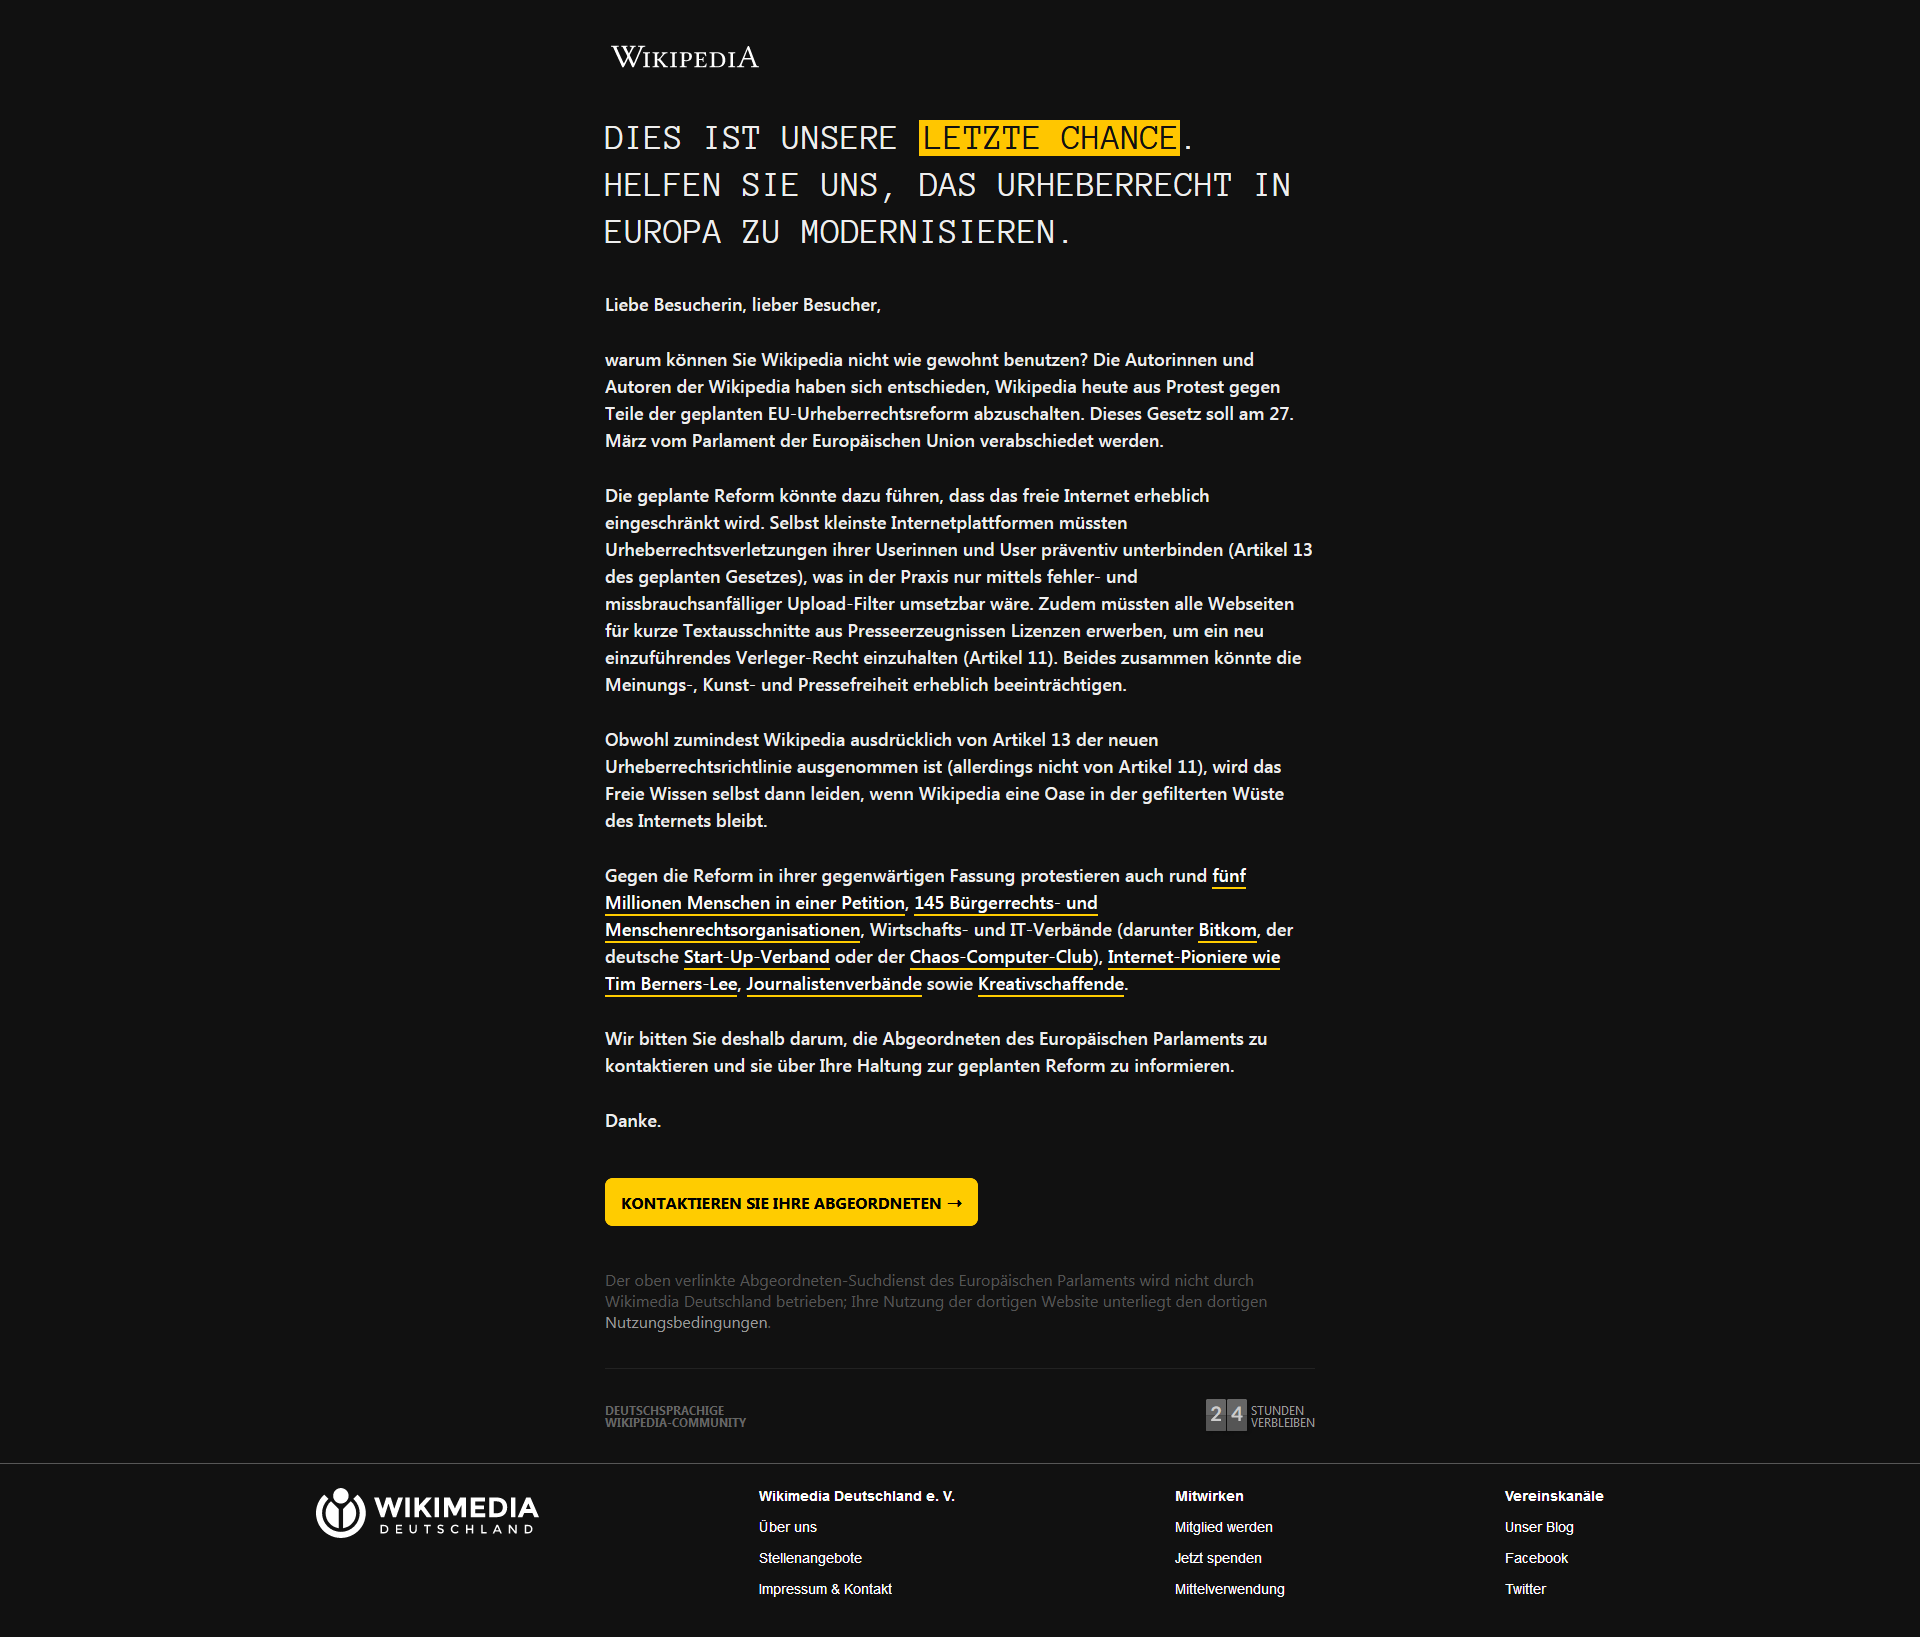
\includegraphics[width=0.9\columnwidth]{pics/Blackout_of_wikipediade_by_Wikimedia_Deutschland_-_March_2019.png}
  \caption{Blackout of wikipedia.de by Wikimedia Deutschland}~\label{fig:blackout-upload-filters}
\end{figure}

via
\url{https://de.wikipedia.org/wiki/Abschaltung_der_deutschsprachigen_Wikipedia_am_21._M%C3%A4rz_2019#/media/File:Blackout_of_wikipedia.de_by_Wikimedia_Deutschland_-_March_2019.png}

see also
\url{https://wikimediafoundation.org/2019/03/20/four-wikipedias-to-black-out-over-eu-copyright-directive/}
"Volunteer editor communities in four language Wikipedias—German, Czech, Danish, and Slovak—have decided to black out the sites on 21 March in opposition to the current version of the proposed EU Copyright Directive.

Those language editions of Wikipedia will redirect all visitors to a banner about the directive, blocking access to content on Wikipedia for 24 hours. "
"These independent language communities decided to black out in the same way most decisions are made on Wikipedia—through discussion and consensus, "

and
\url{https://wikimediafoundation.org/2019/02/28/we-do-not-support-the-eu-copyright-directive-in-its-current-form-heres-why-you-shouldnt-either/}

timeline
\url{https://edri.org/upload-filters-status-of-the-copyright-discussions-and-next-steps/}

\url{https://en.wikipedia.org/wiki/Directive_on_Copyright_in_the_Digital_Single_Market#Positions}

Interesting fact: there are edit filters that try to precisely identify the upload of media violating copyrights

%TODO refer to Lessig, Chapter 10 when making the upload filter commentary

\section{Directions for further studies}
<insert long list of interesting questions here>

\begin{itemize}
	\item Die Zusammenfassung sollte das Ziel der Arbeit und die zentralen Ergebnisse beschreiben. Des Weiteren sollten auch bestehende Probleme bei der Arbeit aufgezählt werden und Vorschläge herausgearbeitet werden, die helfen, diese Probleme zukünftig zu umgehen. Mögliche Erweiterungen für die umgesetzte Anwendung sollten hier auch beschrieben werden.
\end{itemize}



%---------------------------------------------------
%----- Bibliography
%---------------------------------------------------
\phantomsection
\addcontentsline{toc}{chapter}{References}
\bibliographystyle{alpha}
\bibliography{references.bib}


%---------------------------------------------------
%----- Appendix
%---------------------------------------------------
\backmatter
%% ---------------------------------------------------
% ----- Appendix of the template
% ----- for Bachelor-, Master thesis and class papers
% ---------------------------------------------------
%  Created by C. Müller-Birn on 2012-08-17, CC-BY-SA 3.0.
%  Freie Universität Berlin, Institute of Computer Science, Human Centered Computing.
%

\chapter{Appendix}
\label{ch:Appendix}

\section{Code book}
\label{app:code_book}

This section provides a detailed overview of all the codes\footnote{Here, I use the words ``codes'', ``tags'' and ``labels'' interchangeably.} used for the manual tagging of edit filters.
The purpose of the coding was to gain insight into the specific tasks filters are applied for on English Wikipedia.


\begin{longtable}{ | p{5cm} | p{9cm} | }
    \hline
        \multicolumn{2}{|l|}{\textbf{Vandalism}} \\
    \hline
        \multicolumn{2}{|l|}{Structure related} \\
    \hline
    \multirow{2}{*}{avoidant\_vandalism} & According to Wikipedia Vandalism Typology: "Removal of tags such as \verb|{{afd}}| and \verb|{{copyvio}}| in order to conceal deletion candidates or avert deletion of such content. (This does NOT avert deletion. This actually increases the chance that the article will be deleted.); Removal of a \verb|{{speedy deletion}}| tag from an article one created him/herself. Only the \verb|{{hangon}}| tag can be placed there by the creator to avert deletion.; Removal of recent warnings from one's own user talk page of vandalism or other serious violations"~\cite{Wikipedia:VandalismTypes} \\
                                     & Examples: not satisfied with the one thing a dubbed "avoidant\_vandalism?" so far.\\
    \hline
    \multirow{2}{*}{image\_vandalism} & "Uploading shock images that do not belong at all on Wikipedia; Inappropriately placing explicit images legitimately used on Wikipedia on pages where they do not belong"~\cite{Wikipedia:VandalismTypes} \\
                                     & Examples: 952 "Image vandalism IV"; 428 "Image abuse";\\
    \hline
    \multirow{2}{*}{link\_vandalism} & According to Wikipedia Vandalism Typology: "Modifying internal or external links within a page so that they appear the same in the finished version but link to a page/site that they are not intended to (e.g. spam, self-promotion, an explicit image, a shock site, or some other irrelevant page)
    Adding external links to non-notable or irrelevant sites
    Adding spam links
    Adding external links that may belong on another Wikipedia page, but have no relevance to the subject matter of the page to which they are added"~\cite{Wikipedia:VandalismTypes} \\
                               & Examples: none sofar, I do have explicit categories for seo and self promotion..\\ %TODO: do I need this cat? delete?
    \hline
    \multirow{2}{*}{page\_move\_vandalism} & vandalism involving moving a page (i.e. renaming the page), mostly to some nonsensical name
  (Wikipedia typology: "Renaming pages (referred to as "page-moving") to disruptive, irrelevant, or otherwise inappropriate terms.") \\
                               & Examples: 883 "Page moves to bad words or other vandalism"; 334 "Grawp page move vandalism"  \\
    \hline
    \multirow{2}{*}{talk\_page\_vandalism} & Malicious activity taking place at talk pages: e.g. modifiyng or removing other users' comments from discussions \\
                                     & Examples: 842 "Talk page abuse";\\
    \hline
    \multirow{2}{*}{template\_vandalism} & "Modifying a template in a harmful or disruptive manner. This is especially serious, because it'll negatively impact the appearance of multiple pages. Some templates appear on hundreds of pages."~\cite{Wikipedia:VandalismTypes} \\
                                     & Examples: 203 "Template spam from 88.105.0.0/16";\\
    \hline
    \multirow{2}{*}{username\_vandalism} & According to Wikipedia Vandalism Typology ('malicious account creation'): "Creating accounts with usernames that contain deliberately offensive or disruptive terms is considered vandalism, whether the account is used or not."~\cite{Wikipedia:VandalismTypes}; in theory there shouldn't be very many filters of that sort, since there is a username blacklist which would be the more appropriate mechanism to take care of this. \\
                                     & Examples: 827 "Abusive username activity" (unfortunately hidden, so we don't know what the activity is)\\
    \hline \hline
        \multicolumn{2}{|l|}{Content related} \\
    \hline
    \multirow{2}{*}{hoaxing} & deliberately inserting false information (From Wikipedia typology: "Adding plausible misinformation to articles; Use of fictitious references") \\
                                     & Examples: ?\\
    \hline
    \multirow{2}{*}{prank} &  Edit or action is meant as a joke. \\%We probably don't need this, see below for the only filter in this category; also it's also kind of covered by the silly vandalism def (acording to the typology)
                                     & Examples: 396 "Don't delete the main page" (which was never tripped by the way^^)\\
    \hline
    \multirow{2}{*}{} & included during 2nd labeling for marking filters dealing with inserting profanities into articles in general, without them being targeted at a person (that is the difference to 'personal\_attacks') \\
                                     & Examples: ?\\
    \hline
    \multirow{2}{*}{silly\_vandalism} & blatant, immediately obvious vandalism, such as inserting repeating random characters or other intentional nonsence, such as "Baby carrots are yummy in my tummy." (Edit on the Veganism-Page); \\
                                     & Examples: 338 "Vuvuzela vandalism", 135 "Repeating characters"\\
    \hline
    \multirow{2}{*}{trolling} & "Trolling" is explicitely referenced in the filter name;
                                According to \url{https://en.wikipedia.org/w/index.php?title=Internet_troll&oldid=902578463} :
  "In Internet slang, a troll is a person who starts quarrels or upsets people on the Internet to distract and sow discord by posting inflammatory and digressive,[1] extraneous, or off-topic messages in an online community (such as a newsgroup, forum, chat room, or blog) with the intent of provoking readers into displaying emotional responses[2] and normalizing tangential discussion,[3] whether for the troll's amusement or a specific gain. "\\
                                     & Examples: 896 "ANI trolling", 615 "Reference desk trolling"\\
    \hline \hline
        \multicolumn{2}{|l|}{Ideologically motivated} \\
    \hline
    \multirow{2}{*}{politically\_motivated} & Disruptions on explicitely politic matters\\
                                     & Examples: 154 "Macedonia naming conflict 2"; 19 "Replacement of "partition of India" with "independence of Pakistan""\\
    \hline
    \multirow{2}{*}{religiously\_motivated} & Disruptions on topics related to religion\\
                                     & Examples: 131 "Removal of controversial images" (see content; however this could fall under "image\_vandalism" as well)\\
    \hline \hline
        \multicolumn{2}{|l|}{Spam/malware/etc.} \\
    \hline
    \multirow{2}{*}{malware} & Malware is explicitely mentioned in the filter's name \\%TODO maybe combine phishing and malware
                                     & Examples: 243 "WikiMedia Viewer possible malware"; 429 "Possible malware attack" <-- only two instances\\
    \hline
    \multirow{2}{*}{phishing} & Probably stuff that had "phishing" in their name\\
                                     & Examples: 870 "nowiki phishing" <- only instance\\
    \hline
    \multirow{2}{*}{spam} & There is a "Spam" type of vandalism in the Wikipedia Vandalism Typology. However, I've got the feeling that I'm mostly labeling the cases listed there as "self promotion" or similar (although maybe not; This is the def: "    Adding text to any page that promotes an interest that benefits the user, except in user space in a manner allowable under Wikipedia's guidelines
  Alternative: inserting links to promotional content, often not related to the content being edited (from chapter 5)
    Adding external links to site(s) that promote an interest from which the user benefits
    Adding external links to site(s) that have ads from which the user benefits, even if the site has information relevant to the article");
  I've so far labeled "spam" foremost filters which contain the word in their name\\
                                     & Examples: 862 "Arabic string spam";  523 "Page creation spammer";\\
    \hline \hline
        \multicolumn{2}{|l|}{General vandalism} \\
    \hline
    \multirow{2}{*}{bot\_vandalism} & Vandalism caused by an automated agent\\
                                     & Examples: 277 "possible vandalbot"; 276 "scripted anomtalk/spoofed IP vandalism"\\
    \hline
    \multirow{2}{*}{general\_vandalism} & vandalism for which none of the more specific tags applied\\
                                     & Examples: ?\\
    \hline \hline
        \multicolumn{2}{|l|}{Hardcore vandalism (the really malicious cases)} \\
    \hline
    \multirow{2}{*}{abuse} & Filter contains "abuse", "abusive" or similar in its name; \\%TODO do we really need the category
                                     & Examples: ?\\
    \hline
    \multirow{2}{*}{doxxing} & Disclosing private information of other people (e.g. address, contact details, details about their life not know to the public) without their consent; Often with the purpose to facilitate organised harassment and it is thus viewed by Wikipedia as specific form of harassment.
  (According to \url{https://en.wikipedia.org/w/index.php?title=Doxing&oldid=902687406} : "Doxing (from dox, abbreviation of documents)[1] or doxxing[2][3] is the Internet-based practice of researching and broadcasting private or identifying information (especially personally identifying information) about an individual or organization")
Note: according to Wikipedia this behaviour constitutes harassment: "Posting another editor's personal information is harassment, unless that person has voluntarily posted their own information, or links to such information, on Wikipedia. Personal information includes legal name, date of birth, identification numbers, home or workplace address, job title and work organisation, telephone number, email address, other contact information, or photograph, whether such information is accurate or not. " (\url{https://en.wikipedia.org/w/index.php?title=Wikipedia:Harassment&oldid=902881999}) \\
                                     & Examples: 120 "Real life info" (not quite sure though, since filter is hidden)\\
    \hline
    \multirow{2}{*}{harassment} & Filter contains "harassment" in their name/comments
                                  Wikipedia's Policies define harassment (related to Wikipedia) the following way: "[...] stop other editors from enjoying Wikipedia by making threats, repeated annoying and unwanted contacts, repeated personal attacks, intimidation, or posting personal information. [...] "Usually (but not always), the purpose is to make the target feel threatened or intimidated\url{https://en.wikipedia.org/w/index.php?title=Wikipedia:Harassment&oldid=886343748}\\
                                     & Examples: 792 "Harassment"; 330 "Attacks on editors";\\
    \hline
    \multirow{2}{*}{hidden\_vandalism} & Tag for hidden filters where a more specific tag could not be determined\\
                                     & Examples: ?\\
    \hline
    \multirow{2}{*}{impersonation} & Labels filters that target cases where an editor is trying to pose as another editor. Mostly "impersonation" is metioned in the filter name/comments\\
                                     & Examples: 568 "SPI Clerk impersonation";\\
    \hline
    \multirow{2}{*}{long\_term\_abuse} & "The user has been abusing Wikipedia over a long duration of time. The user account has a history of repeated egregious disruption, and despite indefinite block or ban, continues vandalism and/or abuse beyond the point of any usual blocked user." from \url{https://en.wikipedia.org/wiki/Wikipedia:Long_term_abuse}
  Filters that had "Long term abuse" or "LTA" or similar in their name ('af\_public\_comments'); expected to be mostly hidden filters\\
                                     & Example: 51 "LTA Username / LTA IP hopping disruption (Oshwah)"; 937 "Qwertywander long-term abuse";\\
    \hline
    \multirow{2}{*}{not\_polite} & Interaction with others turning non-civil without becoming directly a personal attack? Do we really need this tag if we'll only label one filter with it?\\
                                     & Examples: 521 "Feedback: All caps" (single example)\\
    \hline
    \multirow{2}{*}{personal\_attacks} & Insults directed towards particular persons (be it other editors or persons who are the subject matter of an article)
  \url{https://en.wikipedia.org/w/index.php?title=Wikipedia:No_personal_attacks&oldid=900682398} defines a detailed list of what is considered a personal attack\\
                                     & Examples: 299 "Personal attacks"; 693 "Drake Bell attack";\\
    \hline
    \multirow{2}{*}{sockpuppetry} & Sockpuppetry is the usage of multiple accounts to "mislead, deceive, vandalize or disrupt; to create the illusion of greater support for a position; to stir up controversy; or to circumvent a block, ban, or sanction"~\url{https://en.wikipedia.org/w/index.php?title=Wikipedia:Sock_puppetry&oldid=903464918}
  Filter contains "sock", "sockpuppets", "sockpuppetry" or similar in their name ('af\_public\_comments') or maybe notes ("af\_comments"); expected to be mostly hidden filters (which may have been made public upon deletion or being disabled for example)
  Sockpuppetry is often long term abuse, but not necessarily all long term abuse involves sock puppetry \\
                                     & Examples: 16 "Prolific socker I"; 114 "sleeper socks";\\
    \hline \hline
        \multicolumn{2}{|l|}{} \\
    \hline \hline
        \multicolumn{2}{|l|}{\textbf{Good faith}} \\
    \hline
        \multicolumn{2}{|l|}{Policy violations} \\
    \hline
    \multirow{2}{*}{bad\_style} & Filters targeting edits deviating from what is percieved a good encyclopedic style (def?)\\
                                     & Examples: 899 "Adding "The Sun" or "Dailystar" to BLPs" (presumably, bc they are unreliable sources;); 491 "Edits ending with emoticons or !"; 253 "Signing a non-discussion page"\\
    \hline
    \multirow{2}{*}{copyright\_violation} & Filters targeting potential copyright violations: e.g. images without license information, ..\\
                                     & Examples: 798 "Possible copyvio for image upload"; 278 "Possible copyright violations"\\
    \hline
    \multirow{2}{*}{edit\_warring} & Filters targeting edits that revert each other \\
                                     & Examples: 622 "Genre edit-warring"; 419 "User removing himself from AIV" (first labeling, I would actually simply label this 'vandalism' upon second inspection)\\
    \hline
    \multirow{2}{*}{guideline\_vio} &  Filters target edits violating Wikipedia's guidelines \\%TODO do we need this one and the previous? I would rather merge them.
                                     & Examples: 55 "Signing articles" (which is also labeled 'bad\_style'); it is also the only filter with a 'guideline\_vio' label from the 1st round of labeling\\
    \hline
    \multirow{2}{*}{lazyness} & Slacking on orthography norms (this is something that shouldn't be handled by filters, according to guidelines); smth else?\\
                                     & Examples: 18 "Test type edits from clicking on edit bar" (not quite sure why I have labeled this 'lazyness'); 292 "Repeating characters in edit summary"; 432 "Starting new line with lowercase letters"\\
    \hline
    \multirow{2}{*}{wiki\_policy} & Filters target edits violating Wikipedia's policies\\
                                     & 930 "Prevent indexing userspaces by newer users"; 272 "Page author removing CSD tags"\\
    \hline \hline
        \multicolumn{2}{|l|}{Point of view problems} \\
    \hline
    \multirow{2}{*}{biased\_pov} & Hm.. I have the feeling all the filters here should be relabeled..\\
                                     & Examples: 148 "Users creating autobiographies" (which should be rather "self\_promotion", I think); 894 "Possible Self-Published Sources" (maybe 'self\_promotion' is also more suitable here?); 878 "New user removing COI template"\\
    \hline
    \multirow{2}{*}{conflict\_of\_interest} & Filter targets people editing articles about themselves or organisations they are affilitated to or receive money from.\\
                                     & Examples: 302 "Possible COI"; 588 "Promotional usernames"\\
    \hline
    \multirow{2}{*}{self\_promotion} & specifically promoting one-self, it is kind of part of the 'conflict\_of\_interest'\\
                                     & Examples: 214 "Creating articles with title contained in username" (this is actually one of the 3 filters with this as a label candidate, so I think we can savely merge it with 'conflict\_of\_interest' without significantly losing facettes)\\
    \hline
    \multirow{2}{*}{seo} & Filters targeting SEO edits (mostly, explicitely mentioned in the filter name)\\
                                     & Examples: 36 "SEO push University of Atlanta"; 682 "SEO/Attack page"; 554 "top100 blog charts" (bc of this and the Daily Mail sources, I am contemplating creating a 'unreliable\_sources' label)\\
    \hline \hline
        \multicolumn{2}{|l|}{Structure related} \\
    \hline
    \multirow{2}{*}{good\_faith} & \\
                                     & Examples:\\
    \hline
    \multirow{2}{*}{good\_faith\_article\_creation} & \\
                                     & Examples:\\
    \hline
    \multirow{2}{*}{good\_faith\_categories} & \\
                                     & Examples:\\
    \hline
    \multirow{2}{*}{good\_faith\_deletion} & \\
                                     & Examples:\\
    \hline
    \multirow{2}{*}{good\_faith\_edits} & \\
                                     & Examples:\\
    \hline
    \multirow{2}{*}{good\_faith\_edit\_summary} & \\
                                     & Examples:\\
    \hline
    \multirow{2}{*}{good\_faith\_external\_resources} & \\
                                     & Examples:\\
    \hline
    \multirow{2}{*}{good\_faith\_html} & \\
                                     & Examples:\\
    \hline
    \multirow{2}{*}{good\_faith\_image} & \\
                                     & Examples:\\
    \hline
    \multirow{2}{*}{good\_faith\_move} & \\
                                     & Examples:\\
    \hline
    \multirow{2}{*}{good\_faith\_orthography} & \\
                                     & Examples:\\
    \hline
    \multirow{2}{*}{good\_faith\_redirect} & \\
                                     & Examples:\\
    \hline
    \multirow{2}{*}{good\_faith\_refs} & \\
                                     & Examples:\\
    \hline
    \multirow{2}{*}{good\_faith\_revert} & \\
                                     & Examples:\\
    \hline
    \multirow{2}{*}{good\_faith\_template} & \\
                                     & Examples:\\
    \hline
    \multirow{2}{*}{good\_faith\_test\_edits} & \\
                                     & Examples:18 "Test type edits from clicking on edit bar"\\
    \hline
    \multirow{2}{*}{good\_faith\_userpage} & \\
                                     & Examples:\\
    \hline
    \multirow{2}{*}{good\_faith\_wiki\_links} & \\
                                     & Examples:\\
    \hline
    \multirow{2}{*}{good\_faith\_wiki\_syntax} & \\
                                     & Examples:\\
    \hline
        \multicolumn{2}{|l|}{} \\
    \hline \hline
        \multicolumn{2}{|l|}{\textbf{Maintenance}} \\
    \hline
    \multirow{2}{*}{bug} & Filters targeting software bugs from MediaWiki, browser extensions, etc which sometimes cause eroneous syntax\\
                                     & Examples: 577 "VisualEditor bugs: Strange icons"; 606 "ANI restoration bug";\\
    \hline
    \multirow{2}{*}{general\_maintenance} & Filters taking care of other maintenance tasks (It looks like, I will have problems to distinguish between this one and 'general\_tracking')\\
                                     & Examples: 728 "Huggle"; 942 "Log edits to protected pages"; 199 "Unflagged Bots"\\
    \hline
    \multirow{2}{*}{general\_tracking} & There are various filters introduced with the aim to track certain behaviour in order to determin whether it occurs frequently and how problematic it is\\
                                     & Examples: 362 "New user creating page" would fit better in here I think\\
    \hline
    \multirow{2}{*}{test} & Various test filters (of single edit filter managers or jointly used)\\
                                     & Examples: 398 "Test filter 398"; 358 "Od Mishehu's test filter"; 424 "Repeatedly blocked user --  testing-only rule for filter 425"\\
    \hline \hline
        \multicolumn{2}{|l|}{} \\
    \hline \hline
        \multicolumn{2}{|l|}{\textbf{Unknown}} \\
    \hline
    \multirow{2}{*}{misc} & Cannot fit the filter into any category (it is not that functionality is unclear but I couldn't think of a suitable label)\\
                                     & Examples: 388 "Unusual redirect III" (which is hidden, so according to new def, should be re-labeled "hidden\_vandalism"), 688 "Beals" (same); 708 "SPI page moves"; 152 "External links with referal tags"\\
    \hline
    \multirow{2}{*}{unclear} & I'd say that is similar to misc and both should be merged\\
                                     & Examples: 362 "New user creating page", 300 "Cross-posting"\\
    \hline
    \multirow{2}{*}{unknown} & Cannot determine at all what the filter is doing (but hidden filters with no clear names should be labeled "hidden\_vandalism", since it's pretty clear they target vandalism)\\
                                     & Examples: various; as far as I can see though, all of them are getting re-labeled to "hidden\_vandalism"\\
    \hline
    \caption{Code book}~\label{table:code-book}
\end{longtable}


\section{Extra figures and tables}
\label{app:appendix-figures}

\begin{figure*}
\begin{verbatim}
abuse_filter
+--------------------+---------------------+------+-----+---------+----------------+
| Field              | Type                | Null | Key | Default | Extra          |
+--------------------+---------------------+------+-----+---------+----------------+
| af_id              | bigint(20) unsigned | NO   | PRI | NULL    | auto_increment |
| af_pattern         | blob                | NO   |     | NULL    |                |
| af_user            | bigint(20) unsigned | NO   | MUL | NULL    |                |
| af_user_text       | varbinary(255)      | NO   |     | NULL    |                |
| af_timestamp       | binary(14)          | NO   |     | NULL    |                |
| af_enabled         | tinyint(1)          | NO   |     | 1       |                |
| af_comments        | blob                | YES  |     | NULL    |                |
| af_public_comments | tinyblob            | YES  |     | NULL    |                |
| af_hidden          | tinyint(1)          | NO   |     | 0       |                |
| af_hit_count       | bigint(20)          | NO   |     | 0       |                |
| af_throttled       | tinyint(1)          | NO   |     | 0       |                |
| af_deleted         | tinyint(1)          | NO   |     | 0       |                |
| af_actions         | varbinary(255)      | NO   |     |         |                |
| af_global          | tinyint(1)          | NO   |     | 0       |                |
| af_group           | varbinary(64)       | NO   | MUL | default |                |
+--------------------+---------------------+------+-----+---------+----------------+
\end{verbatim}
  \caption{abuse\_filter schema}~\label{fig:app-db-schemas-af}
\end{figure*}

\begin{figure*}
\begin{verbatim}
abuse_filter_log
+------------------+---------------------+------+-----+---------+----------------+
| Field            | Type                | Null | Key | Default | Extra          |
+------------------+---------------------+------+-----+---------+----------------+
| afl_id           | bigint(20) unsigned | NO   | PRI | NULL    | auto_increment |
| afl_filter       | varbinary(64)       | NO   | MUL | NULL    |                |
| afl_user         | bigint(20) unsigned | NO   | MUL | NULL    |                |
| afl_user_text    | varbinary(255)      | NO   |     | NULL    |                |
| afl_ip           | varbinary(255)      | NO   | MUL | NULL    |                |
| afl_action       | varbinary(255)      | NO   |     | NULL    |                |
| afl_actions      | varbinary(255)      | NO   |     | NULL    |                |
| afl_var_dump     | blob                | NO   |     | NULL    |                |
| afl_timestamp    | binary(14)          | NO   | MUL | NULL    |                |
| afl_namespace    | tinyint(4)          | NO   | MUL | NULL    |                |
| afl_title        | varbinary(255)      | NO   |     | NULL    |                |
| afl_wiki         | varbinary(64)       | YES  | MUL | NULL    |                |
| afl_deleted      | tinyint(1)          | NO   |     | 0       |                |
| afl_patrolled_by | int(10) unsigned    | YES  |     | NULL    |                |
| afl_rev_id       | int(10) unsigned    | YES  | MUL | NULL    |                |
| afl_log_id       | int(10) unsigned    | YES  | MUL | NULL    |                |
+------------------+---------------------+------+-----+---------+----------------+
\end{verbatim}
  \caption{abuse\_filter\_log schema}~\label{fig:app-db-schemas-afl}
\end{figure*}

%TODO do something with the schemas, they are too wide and get cut off on the right side
\begin{figure*}
\begin{verbatim}
abuse_filter_history
+---------------------+---------------------+------+-----+---------+----------------+
| Field               | Type                | Null | Key | Default | Extra          |
+---------------------+---------------------+------+-----+---------+----------------+
| afh_id              | bigint(20) unsigned | NO   | PRI | NULL    | auto_increment |
| afh_filter          | bigint(20) unsigned | NO   | MUL | NULL    |                |
| afh_user            | bigint(20) unsigned | NO   | MUL | NULL    |                |
| afh_user_text       | varbinary(255)      | NO   | MUL | NULL    |                |
| afh_timestamp       | binary(14)          | NO   | MUL | NULL    |                |
| afh_pattern         | blob                | NO   |     | NULL    |                |
| afh_comments        | blob                | NO   |     | NULL    |                |
| afh_flags           | tinyblob            | NO   |     | NULL    |                |
| afh_public_comments | tinyblob            | YES  |     | NULL    |                |
| afh_actions         | blob                | YES  |     | NULL    |                |
| afh_deleted         | tinyint(1)          | NO   |     | 0       |                |
| afh_changed_fields  | varbinary(255)      | NO   |     |         |                |
| afh_group           | varbinary(64)       | YES  |     | NULL    |                |
+---------------------+---------------------+------+-----+---------+----------------+
\end{verbatim}
  \caption{abuse\_filter\_history schema}~\label{fig:app-db-schemas-afh}
\end{figure*}

\begin{figure*}
\begin{verbatim}
abuse_filter_action
+-----------------+---------------------+------+-----+---------+-------+
| Field           | Type                | Null | Key | Default | Extra |
+-----------------+---------------------+------+-----+---------+-------+
| afa_filter      | bigint(20) unsigned | NO   | PRI | NULL    |       |
| afa_consequence | varbinary(255)      | NO   | PRI | NULL    |       |
| afa_parameters  | tinyblob            | NO   |     | NULL    |       |
+-----------------+---------------------+------+-----+---------+-------+
\end{verbatim}
  \caption{abuse\_filter\_action schema}~\label{fig:app-db-schemas-afa}
\end{figure*}

%TODO add column "manual tags" (see jupyter NB)
\begin{table}
  \centering
  \begin{tabular}{r c r }
    % \toprule
    Filter ID & Publicly available description & Hitcount \\ % is the hitcount for the year or altogether till now?-- for the year, of course
    \hline
    135 & repeating characters & 175455 \\
    30 & "large deletion from article by new editors" & 160302 \\
    61 & "new user removing references" ("new user" is handled by "!("confirmed" in user\_groups)") & 147377 \\
    18 & Test type edits from clicking on edit bar & 133640 \\
    3 & "new user blanking articles" & 95916 \\
    172 & "section blanking" & 89710 \\
    50 & "shouting" (contribution consists of all caps, numbers and punctuation) & 88827 \\
    98 & "creating very short new article" & 80434 \\
    65 & "excessive whitespace" (note: "associated with ascii art and some types of vandalism") & 74098 \\
    132 & "removal of all categories" & 68607 \\
    % \bottomrule
  \end{tabular}
  \caption{10 most active filters in 2009}~\label{tab:app-most-active-2009}
\end{table}

\begin{table}
  \centering
  \begin{tabular}{r c r }
    % \toprule
    Filter ID & Publicly available description & Hitcount \\
    \hline
    61 & "new user removing references" ("new user" is handled by "!("confirmed" in user\_groups)") & 245179 \\
    135 & repeating characters & 242018 \\
    172 & "section blanking" & 148053 \\
    30 & "large deletion from article by new editors" & 119226 \\
    225 & Vandalism in all caps & 109912 \\
    3 & "new user blanking articles" & 105376 \\
    50 & "shouting" (contribution consists of all caps, numbers and punctuation) & 101542 \\
    132 & "removal of all categories" & 78633 \\
    189 & BLP vandalism or libel & 74528 \\
    98 & "creating very short new article" & 54805 \\
    % \bottomrule
  \end{tabular}
  \caption{10 most active filters in 2010}~\label{tab:app-most-active-2010}
\end{table}

\begin{table}
  \centering
  \begin{tabular}{r c r }
    % \toprule
    Filter ID & Publicly available description & Hitcount \\
    \hline
    61 & "new user removing references" ("new user" is handled by "!("confirmed" in user\_groups)") & 218493 \\
    135 & repeating characters & 185304 \\
    172 & "section blanking" & 119532 \\
    402 & New article without references & 109347 \\
    30 & Large deletion from article by new editors & 89151 \\
    3 & "new user blanking articles" & 75761 \\
    384 & Addition of bad words or other vandalism & 71911 \\
    225 & Vandalism in all caps & 68318 \\
    50 & "shouting" (contribution consists of all caps, numbers and punctuation) & 67425 \\
    432 & Starting new line with lowercase letters & 66480 \\
    % \bottomrule
  \end{tabular}
  \caption{10 most active filters in 2011}~\label{tab:app-most-active-2011}
\end{table}

\begin{table}
  \centering
  \begin{tabular}{r c r }
    % \toprule
    Filter ID & Publicly available description & Hitcount \\
    \hline
    135 & repeating characters & 173830 \\
    384 & Addition of bad words or other vandalism & 144202 \\
    432 & Starting new line with lowercase letters & 126156 \\
    172 & "section blanking" & 105082 \\
    30 & Large deletion from article by new editors & 93718 \\
    3 & "new user blanking articles" & 90724 \\
    380 & Multiple obscenities & 67814 \\
    351 & Text added after categories and interwiki & 59226 \\
    279 & Repeated attempts to vandalize & 58853 \\
    225 & Vandalism in all caps & 58352 \\
    % \bottomrule
  \end{tabular}
  \caption{10 most active filters in 2012}~\label{tab:app-most-active-2012}
\end{table}

\begin{table}
  \centering
  \begin{tabular}{r c r }
    % \toprule
    Filter ID & Publicly available description & Hitcount \\
    \hline
    135 & repeating characters & 133309 \\
    384 & Addition of bad words or other vandalism & 129807 \\
    432 & Starting new line with lowercase letters & 94017 \\
    172 & "section blanking" & 92871 \\
    30 & Large deletion from article by new editors & 85722 \\
    279 & Repeated attempts to vandalize & 76738 \\
    3 & "new user blanking articles" & 70067 \\
    380 & Multiple obscenities & 58668 \\
    491 & Edits ending with emoticons or ! & 55454 \\
    225 & Vandalism in all caps & 48390 \\
    % \bottomrule
  \end{tabular}
  \caption{10 most active filters in 2013}~\label{tab:app-most-active-2013}
\end{table}

\begin{table}
  \centering
  \begin{tabular}{r c r }
    % \toprule
    Filter ID & Publicly available description & Hitcount \\
    \hline
    384 & Addition of bad words or other vandalism & 111570 \\
    135 & repeating characters & 111173 \\
    279 & Repeated attempts to vandalize & 97204 \\
    172 & "section blanking" & 82042 \\
    432 & Starting new line with lowercase letters & 75839 \\
    30  & Large deletion from article by new editors & 62495 \\
    3 & "new user blanking articles" & 60656 \\
    636 & Unexplained removal of sourced content & 52639 \\
    231 & Long string of characters containing no spaces & 39693 \\
    380 & Multiple obscenities & 39624 \\
    % \bottomrule
  \end{tabular}
  \caption{10 most active filters in 2014}~\label{tab:app-most-active-2014}
\end{table}

\begin{table}
  \centering
  \begin{tabular}{r c r }
    % \toprule
    Filter ID & Publicly available description & Hitcount \\
    \hline
    650 & Creation of a new article without any categories & 226460 \\
    61 & New user removing references & 196986 \\
    636 & Unexplained removal of sourced content & 191320 \\
    527 & T34234: log/throttle possible sleeper account creations & 189911 \\
    633 & Possible canned edit summary & 162319 \\
    384 & Addition of bad words or other vandalism & 141534 \\
    279 & Repeated attempts to vandalize & 110137 \\
    135 & repeating characters & 99057 \\
    686 & IP adding possibly unreferenced material to BLP & 95356 \\
    172 & "section blanking" & 82874 \\
    % \bottomrule
  \end{tabular}
  \caption{10 most active filters in 2015}~\label{tab:app-most-active-2015}
\end{table}

\begin{table}
  \centering
  \begin{tabular}{r c r }
    % \toprule
    % \toprule
    Filter ID & Publicly available description & Hitcount \\
    \hline
    527 & T34234: log/throttle possible sleeper account creations & 437099 \\
    61 & New user removing references & 274945 \\
    650 & Creation of a new article without any categories & 229083 \\
    633 & Possible canned edit summary & 218696 \\
    636 & Unexplained removal of sourced content & 179948 \\
    384 & Addition of bad words or other vandalism & 179871 \\
    279 & Repeated attempts to vandalize & 106699 \\
    135 & repeating characters & 95131 \\
    172 & "section blanking" & 79843 \\
    30 & Large deletion from article by new editors & 68968 \\
    % \bottomrule
  \end{tabular}
  \caption{10 most active filters in 2016}~\label{tab:app-most-active-2016}
\end{table}

\begin{table}
  \centering
  \begin{tabular}{r c r }
    % \toprule
    Filter ID & Publicly available description & Hitcount \\
    \hline
    61 & New user removing references & 250394 \\
    633 & Possible canned edit summary & 218146 \\
    384 & Addition of bad words or other vandalism & 200748 \\
    527 & T34234: log/throttle possible sleeper account creations & 192441 \\
    636 & Unexplained removal of sourced content & 156409 \\
    650 & Creation of a new article without any categories & 151604 \\
    135 & repeating characters & 80056 \\
    172 & "section blanking" & 70837 \\
    712 & Possibly changing date of birth in infobox & 59537 \\
    833 & Newer user possibly adding unreferenced or improperly referenced material & 58133 \\
    % \bottomrule
  \end{tabular}
  \caption{10 most active filters in 2017}~\label{tab:app-most-active-2017}
\end{table}

\begin{table}
  \centering
  \begin{tabular}{r c r }
    % \toprule
    Filter ID & Publicly available description & Hitcount \\
    \hline
    527 & T34234: log/throttle possible sleeper account creations & 358210 \\
    61 & New user removing references & 234867 \\
    633 & Possible canned edit summary & 201400 \\
    384 & Addition of bad words or other vandalism & 177543 \\
    833 & Newer user possibly adding unreferenced or improperly referenced material & 161030 \\
    636 & Unexplained removal of sourced content & 144674 \\
    650 & Creation of a new article without any categories & 79381 \\
    135 & repeating characters & 75348 \\
    686 & IP adding possibly unreferenced material to BLP & 70550 \\
    172 & "section blanking" & 64266 \\
    % \bottomrule
  \end{tabular}
  \caption{10 most active filters in 2018}~\label{tab:app-most-active-2018}
\end{table}



\end{document}
